\chapter{Query templates}\label{template}

% Evaluation of recursive functions
The translated functions follow all a common schema in general. First, the callstack-graph is created, top-down until the basecases are reached. The basecases are then evaluated with the according arguments discovered by the callgraph. Evaluation continues bottom-up as new recursive cases have results of their callsites available.

% Two phases: Callgraph growth and callstack evaluation
This two phases, callstack discovery and callstack evaluation, are implemented by two CTEs, \texttt{callstack} and \texttt{evaluation}. The final query selects the desired final output from the evaluation-CTE. \autoref{fig:standard_template_structure} illustrates the very high level idea of the standard translation template.

\begin{figure}[h!]
    \centering
    \sqlcode{snippets/template_structure.sql}
    \caption{High-level structure of the standard query template (simplified).}
    \label{fig:standard_template_structure}
\end{figure}

% Special care needs to be taken to behave not only in terms of result values, but also in terms of termination.
Special care needs to be taken to behave like the original function in terms of termination. Call-loops in the original function lead to an infinite growing callstack, causing nontermination. By using memoization in the translation, this does not happen in our template, so we have to detect that case and manually init nontermination.

In this chapter I will provide a number of "macros" that fill the templates with values. I give these macros with respect to the running example of \texttt{fib}, so for a function with a single attribute. This avoids cluttering difficult spots with excessiv notation. To generalize to more attributes the following things need to be done:
\begin{itemize}
    \item Instead of a single column \texttt{in\_1} or \texttt{out\_1}, we need further columns \texttt{in\_2, ..., in\_n} and \texttt{out\_2, ..., out\_n}.
    \item Whenever we match tables by their arguments, eg. \texttt{(c.in\_1) = (e.out\_1)} it is clear that this needs to be altered analogous to \texttt{(c.in\_1, c.in\_2, ..., c.in\_n) = (e.out\_1, e.out\_2, ..., out\_n)}.
    \item The same applies whenever replacing UDF arguments: \texttt{q[x1/\$1]} needs to become \texttt{q[x1/\$1, x2/\$1, ..., xn/\$n]}.
\end{itemize}
For full examples with more than one argument see the appendix. 

\section{Callgraph discovery}

The idea of the callgraph-CTE is to utilize the generated predicates from the recursive scenarios to detect which callsites in the original query are reached with the arguments of the current invocation.
Starting with the original arguments of the UDF-invocation the applicable scenario is detected and the contained callsites are discovered. The arguments passed to the newly discovered callsites are evaluated independetly and used to recursively collect subsequent calls.

\subsection{Tabular callgraph representation}

\begin{figure}[h!]\small
    \begin{minipage}[b]{.5\linewidth}
    \centering
    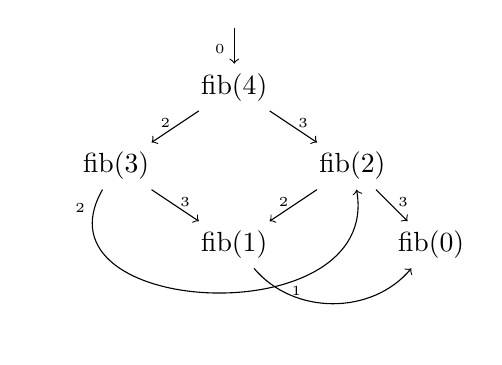
\begin{tikzpicture}
% nodes
\node (f4)     at (2.5, 2) {fib(4)};
    \node (f3) at (1, 1) {fib(3)};
        \node (f1) at (2.5, 0) {fib(1)};
    \node (f2) at (4, 1) {fib(2)};
        \node (f0) at (5, 0) {fib(0)};
% arrows
\draw[<-] (f4) -- node[pos=0.4, left, label distance=5mm]{\tiny{0}} +(0, 0.75);

\draw[->] (f4) -- node[pos=0.4, left, label distance=5mm]{\tiny{2}} (f3);
\draw[->] (f4) -- node[pos=0.4, right, label distance=5mm]{\tiny{3}} (f2);

    \draw[->, bend right=100, out=240, looseness=1.5] (f3) to node[pos=0.05, left, label distance=5mm]{\tiny{2}} (f2);
    \draw[->] (f3) -- node[pos=0.4, right, label distance=5mm]{\tiny{3}} (f1);
    \draw[->] (f2) -- node[pos=0.4, left, label distance=5mm]{\tiny{2}} (f1);
        \draw[->, bend right=50] (f1) to node[pos=0.2, right, label distance=5mm]{\tiny{1}} (f0);
    \draw[->] (f2) -- node[pos=0.4, right, label distance=5mm]{\tiny{3}} (f0);
\end{tikzpicture}
    \subcaption{Callgraph during execution}\label{fig:fib_callstack_graph}
    \end{minipage}%
    \begin{minipage}[b]{.5\linewidth}
    \centering
     
    \begin{tabular}{c|c|c}
        \texttt{in\_arg\_1} & \texttt{callsite} & \texttt{call\_arg\_1} \\
        \hline
        \hline
        \texttt{NULL} & \texttt{0} & \texttt{4}\\
        \texttt{4} & \texttt{2} & \texttt{3}\\
        \texttt{4} & \texttt{3} & \texttt{2}\\
        \hline
        \hline
        \texttt{3} & \texttt{2} & \texttt{2}\\
        \texttt{3} & \texttt{3} & \texttt{1}\\
        \texttt{2} & \texttt{2} & \texttt{1}\\
        \texttt{2} & \texttt{3} & \texttt{0}\\
        \hline
        \texttt{1} & \texttt{1} & \texttt{0}\\
        \hline
    \end{tabular}
    \subcaption{Tabular representation of the callstack}\label{fig:fib_callstack_table}
    \end{minipage}
    \caption{Callgraph of \texttt{fib(4)} (a) and its tabular representation as generated by the \texttt{callstack}-CTE (b). Each edge represents a callsite.}\label{fig:fib_callstack}
\end{figure}

The callstack-CTE creates a direct encoding of the callstack graph (\autoref{fig:fib_callstack}). Each row depicts an edge between two nodes, including the label. Nodes of the callgraph correspond to recursive invocations, identified by their arguments, one column per argument. Beside arguments of the caller and callee, the id of the callsite is noted. Callsite ids are used to associate callsites to scenarios.

\subsection{Collecting callsite arguments}

Thanks to the data from the scenario analysis, the query to add the rows for new callsite can be generated by a simple macro (\autoref{marco:collect_call_maybe}). The predicate acts as guard to add only callsites of the appropriate evaluation scenario. Only if the predicate is fulfilled, any row is returned. The third row in \autoref{fig:fib_callstack_table} is eg. generated by \mintinline{postgresql}{<collect_call_maybe(d.out_1, p1, <callsite id: 2, arg_1: (SELECT $1 - 2)>)>}.

\begin{figure}[h!]\centering
    \begin{minted}{postgresql}
    <collect_call_maybe(in_arg_1, predicate, callsite)>
        := SELECT
             in_arg_1                    AS in_1, 
             callsite.id                 AS callsite_id,
             callsite.arg_1[in_arg_1/$1] AS out_1
           FROM predicate AS p(is_true)
           WHERE p.is_true
    \end{minted}
  \caption{Pseudocode to generate a single call to the callgraph-table. $q[y/x]$ denots the operation of replacing y for x in q. For \texttt{in\_arg\_1} it is used in the beginning \$1 and later references to preceding arguments from the table.}
  \label{marco:collect_call_maybe}
\end{figure}

The macro from \autoref{marco:collect_call_maybe} creates only a query, returning one or none rows. To collect \textit{all} callsites, the query needs to test all callsites of all scenarios (\autoref{macro:collect_calls}). As all callsites within a scenario depend on the same predicate, the scenario-predicate can be pulled up into a CTE to avoid multiple evaluations.

\begin{figure}[h!]\centering\small
    \begin{minted}{postgresql}
    <collect_calls(in_arg_1, scenarios)> :=
        WITH p1 AS (scenarios[1].predicate)[in_arg_1/$1],
             p2 AS (scenarios[2].predicate)[in_arg_1/$1]
             
        -- Scenario 1
        (   -- Callsite 1
            <collect_call_maybe(in_arg_1, p2, scenarios[2].callsites[1])>   )
        
        UNION
        
        -- Scenario 2
        (   -- Callsite 2
            <collect_call_maybe(in_arg_1, p1, scenarios[1].callsites[1])>
          UNION
            -- Callsite 3
            <collect_call_maybe(in_arg_1, p1, scenarios[1].callsites[2])>   )
\end{minted}
  \caption{All callsites of all scenarios needs to be tested to cover the entire function.}
  \label{macro:collect_calls}
\end{figure}

With the query generated by \texttt{<collect\_calls(\$1, scenarios)>} all callsites of the initial UDF invocation are obtained. Subsequent levels of the callgraph can be collected recursively by using the \texttt{out\_1}-column from the previous iteration instead of \texttt{\$1}. For each callsite from the previous iteration, the according evaluation scenario needs to be detected to collect new callsites. This for-each behaviour is implemented by \texttt{LATERAL} in the marco for \texttt{callgraph}.

\begin{figure}[h!]\centering
\begin{minted}{postgresql}
<callstack(rec_scenarios)> :=
  (
    (SELECT NULL, 0, $1) -- add original call
      UNION ALL
    <collect_calls($1, rec_scenarios)> 

  ) UNION (
    SELECT
      new_calls.*
    FROM
      callstack AS c, LATERAL (
        <collect_calls(c.out_1, rec_scenarios)>
      ) AS new_calls
  )
\end{minted}
  \caption{}
  \label{}
\end{figure}

For a complete example of the \texttt{callgraph}-CTE for fib, see \autoref{fib:callstack_cte_complete} in the appendix.

Callgraph growth ends as soon as no recursive scenario is applicable for any newly discovered callsites, ie. all callsites lead to basecases. In this case, the new iteration contains no rows, making \texttt{WITH RECURSIVE} stop.

\section{Callgraph evaluation}
% Evaluation starts bottom up at the leaves of the callstack
Evaluation starts bottom up from the leafs of the callgraph. Scenarios are evaluated by replacing their original arguments with references to the arguments from the callgraph (\autoref{macro:single_basecase}). Scenarios may depend on other scenarios that need to be evaluated first. If all dependencies of a scenario are evaluated, the scenario can be evaluated itself. Nonrecursive scenarios have no dependencies by definition and can be evaluated therefore straight ahead. From this initial rows evaluation continues. Finally, the desired result can be selected.

\begin{figure}[h!]\small
    \begin{minipage}[b]{.45\linewidth}
    \centering
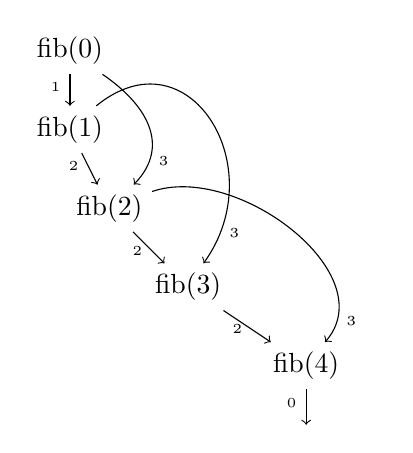
\begin{tikzpicture}
% nodes
\node (n4) at (2.5, -2) {fib(4)};
\node (n3) at (1, -1) {fib(3)};
\node (n2) at (0, 0) {fib(2)};
\node (n1) at (-0.5, 1) {fib(1)};
\node (n0) at (-0.5, 2) {fib(0)};
% arrows
\draw[->] (n0)     to node[pos=0.4,left] {\tiny{1}} (n1);
\draw[->, bend left=40, looseness=1.2, in=120] (n0)     to node[pos=0.8,right] {\tiny{3}} (n2);
\draw[->] (n1)     to node[pos=0.4,left] {\tiny{2}} (n2);
\draw[->, bend left=70, looseness=1.6, out=95] (n1)     to node[pos=0.9,right] {\tiny{3}} (n3);
\draw[->] (n2)     to node[pos=0.6,left] {\tiny{2}} (n3);
\draw[->, bend left=60, looseness=1, in=90] (n2)     to node[pos=0.9,right] {\tiny{3}} (n4);
\draw[->] (n3)     to node[pos=0.6,left] {\tiny{2}} (n4);
\draw[->] (n4)     to node[pos=0.4,left] {\tiny{0}} +(0, -0.75);
\end{tikzpicture}
    \subcaption{}\label{}
    \end{minipage}%
    \hfill
    \begin{minipage}[b]{.45\linewidth}
    \centering
    \begin{tabular}{c|c}
        \texttt{in\_arg\_1} & \texttt{result}\\
        \hline
        \hline
        \texttt{0} & \texttt{0}\\
        \hline
        \hline
        \texttt{1} & \texttt{1}\\
        \hline
        \texttt{2} & \texttt{1}\\
        \hline
        \texttt{3} & \texttt{2}\\
        \hline
        \texttt{4} & \texttt{3}\\
        \hline
    \end{tabular}
    \subcaption{}\label{fig:fib_callstack_cte}
    \end{minipage}
    \caption{a) Dependency-graph, directly retrieved from the callgraph. Callsite ids are annotated to the edges. Leafs are callsites resulting in basecases. b) \texttt{evaluation}-table that holds results for all evaluated scenarios. The first row is the result of the basecase. Following rows are computed iterativly.}\label{}
\end{figure}

\subsection{Evaluating nonrecursive scenarios}
Arguments for the evaluation of nonrecursive scenarios can be found in the leafs of the callgraph.
Evaluation of a single scenario is rather simple. UDF-arguments like \texttt{\$1} are replaced by references to arguments from the callgraph. The predicate from the generated scenario is evaluated in the \texttt{WHERE}-clause and prevents evaluation of wrong scenarios. \autoref{macro:single_basecase} shows a macro for evaluating a single scenario. Each scenario corresponds to a single query returning one or no rows. To collect all scenarios the union of this queries is built.
\begin{figure}[h!]
    \centering
    \begin{minted}{postgresql}
<evaluate nonrecursive scenario(scenario)>
 := SELECT c.out_1                    AS in_1, 
           scenario.query[c.out_1/$1] AS result
    FROM calls_to_basecase c
    WHERE scenario.predicate[c.out_1/$1]
    \end{minted}
    \caption{Macro for nonrecursive scenario evaluation.}
    \label{macro:single_basecase}
\end{figure}

For efficiency, nodes of recursive scenarios are filtered from the callgraph (resulting in CTE \texttt{calls\_to\_basecase}) as they cannot belong to basecases. If a callsite with argument \texttt{out\_1} can be found as input argument \texttt{in\_1} in the callgraph, then \texttt{out\_1} belongs to a recursive scenario. Graphically speaking, the query selects nodes of the callgraph with no outgoing edges, namely leafs, which represents callsites that leads to basecases.

\begin{figure}[h!]
    \centering
    \begin{minted}{postgresql}
<basecases(scenarios)> := 
   WITH calls_to_basecase(out_1) AS (
       SELECT DISTINCT out_1 
       FROM callgraph AS c
       WHERE NOT EXISTS (SELECT NULL FROM callgraph AS c2
                         WHERE c2.in_1 IS NOT DISTINCT FROM c.out_1)
   )
   <evaluate scenario(scenario[1], calls_to_basecases)>
     UNION ALL 
   <evaluate scenario(scenario[2], calls_to_basecases)>
    \end{minted}
    \caption{\texttt{basecase}-CTE.}
    \label{macro:basecases}
\end{figure}

The awkward \texttt{WHERE}-clause stirs from two issues. First, \texttt{IS NOT DISTINCT FROM} is the SQL-way of writing a simple \textit{=} while considering \mintinline{postgresql}{NULL=NULL} as true. This is required since \texttt{NULL} can be an argument of a callsite and needs to be matched with its result-row - tri-state logic hinders that. The \texttt{NOT EXISTS} comes from the fact that the simpler \texttt{NOT IN} is executed for every row as a subquery while \texttt{NOT EXISTS} is executed as a much more efficient antijoin. If disregarding this two issues, the \texttt{WHERE}-clause could be written easier to understand as \mintinline{postgresql}{c.out_1 NOT IN (SELECT c2.in_1 FROM callgraph c2)}.


\subsection{Recursive scenario evaluation}
The evaluation of recursive scenarios follows the schema of the evaluation of nonrecursive scenarios, but is a bit more involved. Callsite-results must be collected per scenario to decide if the scenario is evaluable yet. Only if all callsites of a scneario are evaluated, the scenario can be evaluated itself.

This operation resembles relational divsion $\texttt{S} \div \texttt{R}$: When dividing \texttt{S} by \texttt{R}, table \texttt{S} is grouped by the attributes that are not involved as join-attributes with \texttt{R}. The grouped columns from \textit{S} are returned, if every row in the group have found a join-partner from \texttt{S}. By dividing \texttt{callgraph} by \texttt{evaluation} (projecting away \texttt{callgraph.call\_site\_id}), we obtain only those input arguments that are evaluable, ie. have all required callsite-results available.

\begin{wrapfigure}{r}{0.6\textwidth}
  \sqlcode{snippets/relational_division.sql}
  \caption{Selecting available callsite-results per scenario using relational division with \texttt{array\_agg}. Does not play well with array-arguments.}
  \label{relational_division}
\end{wrapfigure}

The difficulty is to collect those callsite-results. The intuitive approach is to add an \texttt{array\_agg(e.result)} to the relational division (\autoref{relational_division}) that collects the results per scenario. This works well as long as we do not allow arrays as arguments: \texttt{array\_agg} require all input arrays to have the same dimensionality.

The solution is to avoid array aggregation and to "pivot" the groups instead: each callsite-result gets its own column. Pivoting is implemented by using Window-Functions and Partitions together with \texttt{nth\_value} instead of \texttt{GROUP BY} and \texttt{array\_agg}. This way, we circumvent any constraints regarding arrays and avoid expensive aggregation.

\vspace{5mm}

With this problem solved, evaluating a recursive scenario boiles down to replacing UDF-arguments and callsites with \texttt{callgraph}- resp. \texttt{evaluation}-references, similar to the evaluation of nonrecursive scenarios (\autoref{macro:single_basecase}). \autoref{macro:recursive_scenario_evaluation} gives a macro to evaluate a scenario utilizing the pivoting approach from above.

\begin{figure}[h!]\small
    \centering
    \begin{minipage}[b]{\linewidth}
    \centering
    \sqlcode{snippets/eval_recursive_scenario.sql}
    \vspace{3mm}
    \subcaption{(b) shows the result of the join, (c) the final result of the generated query and the effects of the ~\WHERE-clauses are annnotated: \circled{1} Do not consider arguments already evaluated callsites. \circled{2} Only consider callsites of the given scenario we are about to evaluate. \circled{3} Only keep rows where all callsites have an result available.}\label{}
    \end{minipage}%
    \vspace{7mm}
    \begin{minipage}[b]{\linewidth}
    \centering
    \begin{tabular}{c|c|p{10cm}p{1em}p{1cm}|c}
      \multicolumn{3}{l}{$\overbrace{\rule{5.2cm}{0pt}}^{\texttt{callgraph}}$}  & ${}^{\bowtie}$ & \multicolumn{2}{l}{$\overbrace{\rule{2.8cm}{0pt}}^{\texttt{evaluation}}$} \\
      \texttt{c.in\_1}                        & \texttt{c.call\_site\_id}  & \multicolumn{3}{c|}{\texttt{c.out\_1 = e.in\_1}} & \texttt{e.res}                                         \\\hline
      \multirow{2}{*}{\color{gray}4}          & \color{gray}2              & \multicolumn{3}{c|}{\color{gray}3}               & \texttt{\color{gray}NULL} \\
                                              & \color{gray}3              & \multicolumn{3}{c|}{\color{gray}2}               & \color{gray}1             \\\hline
      \cellcolor{green!25}                    & \cellcolor{yellow!30}2     & \multicolumn{3}{c|}{2}                           & \cellcolor{blue!20}1             \\
      \cellcolor{green!25}\multirow{-2}{*}{3} & \cellcolor{yellow!30}3     & \multicolumn{3}{c|}{1}                           & \cellcolor{red!20} 1            \\\hline
      \multirow{2}{*}{\color{gray}2}          & \color{gray}2              & \multicolumn{3}{c|}{\color{gray}1}               & \color{gray}1             \\
                                              & \color{gray}3              & \multicolumn{3}{c|}{\color{gray}0}               & \color{gray}0             \\\hline
      \color{gray}1                           & \color{gray}1              & \multicolumn{3}{c|}{\color{gray}0}               & \color{gray}0             \\\hline
    \end{tabular}
    \subcaption{Callgraph table joined with evaluation table.}\label{}
    \end{minipage}%
    \vspace{7mm}
    \begin{minipage}[b]{\linewidth}
    \centering
    \begin{tabular}{rc|c|c|c}
          & \texttt{in\_1} & \texttt{call\_1} \footnotesize{\color{gray}(id: \colorbox{yellow!20}{2})}  & \texttt{call\_2} \footnotesize{\color{gray}(id: \colorbox{yellow!20}{3})} & \texttt{count} \\\cline{2-5}
         \circled{3}                          & \color{gray}\markForTikz{row1Start}{4} & \color{gray}\texttt{NULL}                  & \color{gray}1                     & \color{gray}\markForTikz{row1End}{1} \\\cline{2-5}
         & \cellcolor{green!25}3              & \cellcolor{blue!20}1 & \cellcolor{red!20}1 & 2                                                            \\\cline{2-5}
         \circled{1}                          & \color{gray}\markForTikz{row2Start}{2} & \color{gray}1                              & \color{gray}0                     & \color{gray}\markForTikz{row2End}{2} \\\cline{2-5}
         \circled{2}                          & \color{gray}\markForTikz{row3Start}{1} & \color{gray}1                              & \color{gray}0                     & \color{gray}\markForTikz{row3End}{1} \\\cline{2-5}
    \end{tabular}
    \DrawHLine[thick, opacity=0.5]{row1Start}{row1End}
    \DrawHLine[thick, opacity=0.5]{row2Start}{row2End}
    \DrawHLine[thick, opacity=0.5]{row3Start}{row3End}
    \subcaption{Result of the query. Rows filtered by \WHERE~ are striked through,}\label{}
    \end{minipage}%
    \caption{Collecting callsite results of for evaluation of a scenario. The result for \texttt{fib(3)} is beeing evaluated. Table (a) shows the result of the }\label{macro:recursive_scenario_evaluation}
\end{figure}

The self-reference in recursive CTEs contains only the rows from the previous iteration, which is a problem when evaluating. Take the evaluation of \texttt{fib} for example (see \autoref{fig:fib_callstack_graph}): Each recursive scenario depends on the results from the last (\texttt{fib(n-1)}) and the penultimate iteration (\texttt{fib(n-2)}). Standard recursive CTE-semantics allows only access to \texttt{fib(n-1)}.

To work around this restriction, the working table is added to the actual result-rows in each iteration. If we choose this approach, the working-table will be never empty, but an empty working-table is the stopping criterion for evaluation of the CTE. Therefore we need to manually take care of returning an empty table when evaluation should stop. To achieve this, the new rows are computed seperately in a CTE and guard also addition of the previous results. \autoref{macro:evaluation_cte}, that shows the final \texttt{evaluation}-CTE, implements this approach.

\begin{figure}[h!]
  \sqlcode{snippets/evaluation_cte.sql}
  \caption{High-level structure of the evaluation-CTE}\label{macro:evaluation_cte}
\end{figure}


\FloatBarrier
\subsection{Result collection and termination}

The previous section introduced the components required to start and continue evaluation of recursive scenarios. The final task is to select the result or to trigger an infinite loop if a setting is detected where the original UDF does not terminate, but the translation has.

There are two ways how a recursive function may not terminate: Infinite recursion and looping calls. Infinite recursion leads always to new calls, never reaching a basecase, the callgraph is infinite. Each new call results in a new, different row that is added to the callgraph-table (\autoref{fig:infinite_callstack}). In this case, the translation does not terminate correctly, as the original.

\begin{figure}[h!]\small
    \begin{minipage}[b]{.5\linewidth}
    \centering
    \begin{minted}{sql}
SELECT CASE WHEN n = 0 THEN 0
            ELSE f(n-2)
       END
    \end{minted}
    \subcaption{UDF-body of a function \texttt{f}}
    \label{fig:infinite_callstack_udf}\par\vfill
    \end{minipage}%
    \begin{minipage}[b]{.5\linewidth}
    \centering
    \begin{tabular}{c|c|c}
in\_n & callsite & param\_n \\\hline
3  & 1 &  1 \\
1  & 1 & -1 \\
-1 & 1 & -3 \\
-3 & 1 & -5 \\
$\vdots$ & $\vdots$ & $\vdots$
    \end{tabular}
    \subcaption{Callgraph of that function. Recursion without a basecase.}
    \label{fig:infinite_callstack_callstack}
    \end{minipage}
    \caption{The function misses its basecase if called with an odd number like 3 and does not terminate. Every call leads to a new, different recursive call as call-arguments grow towards infinity.}\label{fig:infinite_callstack}
\end{figure}

The other case is looping calls. Since we utilize memoization, redundant calls lead only to a single row in the callgraph-table and not to multiple identical rows. Thus, the callgraph-table is finite while the original callgraph is not. Therefore, our implementation would terminate while the original does not. To maintain the original UDf behaviour we need to detect this case and trigger an infinite loop manually.

\begin{figure}[h!]\small
    \begin{minipage}[b]{.45\linewidth}
    \centering
    \begin{minted}{sql}
SELECT CASE WHEN n = 0 THEN 0
            WHEN n = 2 THEN f(0)
            ELSE f(n % 2) + f(2)
       END
    \end{minted}
    \subcaption{}\label{fig:some_loop_udf}
    \end{minipage}%
    \begin{minipage}[b]{.3\linewidth}
    \centering
    \begin{tabular}{c|c|c}
in\_n & callsite & param\_n \\\hline
3 & 2 & 1 \\
3 & 3 & 2 \\
2 & 1 & 0 \\
1 & 2 & 1 \\
1 & 3 & 2
    \end{tabular}
    \subcaption{}\label{fig:some_loop_callstack}
    \end{minipage}
    \begin{minipage}[b]{.2\linewidth}
    \centering
    \begin{tabular}{c|c}
in\_n & result \\\hline
0 & 0 \\\hline
2 & 0 \\
    \end{tabular}
    \subcaption{}\label{fig:some_loop_evaluation}
    \end{minipage}
    \caption{a) UDF-body of a function \texttt{f} where only some part of the callstack causes a loop. b) The callstack is finit, due to memoization. c) Evaluation can start, because some basecases are present, but has not all results available to finish evaluation up to the original call-arguments \texttt{3}.}\label{fig:some_loop}
\end{figure}

How is this situation detectable? If at least one path in the callgraph contains a loop, this path have no basecase where evaluation could start and thus evaluation will stop eventually without having evaluated the root-node. There is no row in the \textit{evaluation}-CTE containing a result for the original UDF-arguments. Instead of returning an empty table, an infinite loop is triggered (\autoref{fig:some_loop}).


\begin{figure}[h!]
    \centering
    \sqlcode{snippets/result_collection.sql}
    \caption{}
    \label{macro:result_collection}
\end{figure}


\chapter{Analysis rules}

% Intuition how scenario analysis works, then formal inference rules are presented
% Begin with four rules to translate the core of each recurisve UDF
% Extending scope to whole queries
% Adding CTEs
% Post processing


Implementing a complex algorithmic idea straight away and refining it while implementing is difficult. The implementation is always just an encoding of an abstract idea, cluttered with language-specific details. Thus, we use abstract inference rules to formalize the idea of slicing a query into its evaluation scenarios. This rules are implemented very closely in the Haskell implementation.

This chapter gives detailed insights of how a given query is sliced into its scenarios and predicates by presenting inference rules. Before introducing the actual formal rules, I will first give an intuition of how the translation idea for each language construct works, before formalizing it.

I begin with presenting a set of four rules that are required to translate simple \CASE-expressions. The nonrecursive rules \RREC und \RBASE handle the case when the SQL-fragment is directly a recursive call resp. does not contain any call at all. Disassembling \CASE-expressions is the true core of the translation process as it is the origin of any scenario. Each \WHEN-\THEN~branch is processed step by step by the \RWHEN-rule and eventually the \ELSE-branch by the \RELSE-rule.

To translate expressions and whole queries four further rules are required that all boil down to a common idea. This idea is that functions have a number of recursive operands that can be translated independently from each other. The different combinations of argument-scenarios form different scenarios of the function itself. Functions in this context can not only be actual functions like \texttt{+}, \texttt{GREATEST} or \texttt{fib}), but also any syntactic construct (eg. \texttt{IS BETWEEN}, \texttt{INNER JOIN}, \texttt{UNION}) that can be understood as one computation step with independant arguments. This schema is also applicable for select- and from-clauses.

Finally, we allow the use of CTEs that come with a couple of complexities. Due to CTEs, it is possible that a recursive SQL-fragment does not contain a callsite directly but indirect via referenced CTEs. Furthermore, CTEs can reference other CTEs so it is necessary to track CTE-dependencies and maintain a list of recursive CTEs while taking shadowing into account.

Before the templates can be finally filled, each scenario needs to be enriched with some information. A data-structure is the template-macros use to create the final templates. As a part of this, callsite-arguments are extracted from each callsite in every scenario. I provide a set of inference rules that perform this task while handling CTE the same way as in the rules for scenario generation.

\section{Preliminaries}\label{approach}

\subsection{Structural Operational Semantics}

A Structural Operational Semantic is an abstract way to define program evaluation step by step. Formally stated, it defines relations between states of an abstract machine. A state $S = (E, c)$ consists of an environment $E$ and some "code" $c$. Relations define transitions between two states. The notation $S \rightarrow S'$ (read: "$S$ evaluates \textit{in one step} to $S'$") is so just a shorthand for $(S, S') \in \rightarrow$ where $\rightarrow$ is the relation. In my rules, the environment does not change during a rule application so we can shorten notation and write $E \vdash c \rightarrow c'$. \cite[Chapter 2]{semanticsWithApplications}

A rule may have a number of \textit{premises} $p_1, p_2, \dots, p_n$ that must hold for the rule to be applicable. This premises are written on top of a line above the rule. This premises may include \textit{judgments} over transitions $T \rightarrow* T'$, that depict that two states are element of the reflexive transitive closure of the relation, ie. that $T$ can be evaluated to $T'$.

$$\quad(\textsc{rule})\inferrule{
   p_1\\
   p_2\\
   \dots\\
   p_n
}{
    S \rightarrow S'
}$$

Evaluation happens by recursively applying transition rules from a starting state. Premises that include judgments causes a callstack to build up until an axiom returns eventually a result (right part of the arrow). In the context of analyzing queries, many premises analyze a part of the query and than wraps the result into its own structure.

The provided rules give deterministic evaluation steps, ie. at most one rule is applicable at a time. This makes the rules a bit more verbose, but simplifies implementation as no backtracking need to be implemented to find the applicable rule.

In the case of the scenario analysis, the state is $(C, T, q, r)$. $C$ is a store used for CTEs that works like a hash-map${}^+$. $C[a, b]$ returns the CTEs from the store with alias $a$ and $b$, if present. The empty CTE-store is denoted as $\varnothing$. $T$ is a set of table-references in scope that are recursive. $q$ is the input query and $r$ is the result of the analysis. $C$ and $T$ are taken as environment. An analysis result $r$ with three scenarios could like this:
$$
\Big(
    \overbrace{\big\{
        \underbrace{
            (p_1, q_1)
        }_{\text{scenario 1}}
    \big\}}^{\text{basecase scenarios}}
    ,
    \overbrace{\big\{
        \underbrace{
            (p_2, q_2)
        }_{\text{scenario 2}},
        \underbrace{
            (p_3, q_3)
        }_{\text{scenario 3}}
    \big\}}^{\text{recursive scenarios}}
\Big)
$$

\subsection{Subset of SQL}
Rules to analyze arbitrary queries would need to consider every single language construct. Instead, we focus on a smaller subset of SQL (\autoref{lst:sql_grammar}) to keep the number of rules small and demonstrate the core idea. Generalizations can be added easilly later. The grammar describes nested WITH-SELECT-FROM-WHERE queries with query-combining functions.

Functions in the grammar are stated in praefix-notation, even if the actual function comes in the form of eg. \texttt{i IS BETWEEN a AND b}, \texttt{x[n]} or \texttt{a IN (<query>)}. Those syntactic details are not visible when represented as AST and all constructs that act like a function are considered a function during translation.

\begin{figure}[H]
    \begin{minted}{postgresql}
    <query>     ::= [ WITH (<query>) AS <tblAlias>[, ...] ]
                      SELECT [ DISTINCT ] <expr>  AS <colAlias>[, ...]
                    [ FROM <tbl>     AS <tblAlias>[, ...] ]
                    [ WHERE <expr> ]
                 |  <query> { UNION | INTERSECT | EXCEPT } [ALL] <query>
    <tbl>       ::= <tblRef> | (<query>) | <fun>([<expr>, ...])
    <expr>      ::=  <const> |  <colRef> |  <fun>([<expr>, ...])
                 |  CASE [WHEN <expr> THEN <expr>, ...] ELSE <expr> END
                 |  ( <query> )
    <fun>       ::= Stable functions
    <const>     ::= SQL built-in constants
    <tblAlias>  ::= alias(colAlias[, ...])
    <colAlias>  ::= alias
    \end{minted}
    \caption{The subset of SQL that is targeted by the inference rules.}
    \label{lst:sql_grammar}
\end{figure}


%\subsection{No VOLATILE functions}
%Without referential transparancy we cannot assume that two function calls within the same query return the same value, making it impossible to use memoization. Therefore, only UDFs markes as STABLE or IMMUTEABLE (38.7. Function Volatility Categories) are translateable.
%Since we use \texttt{UNION} during the evaluation-phase, the rows are checked on equality. This confronts us with a quirk of PostgreSQL: Composite types have no built in function to check equality, thus \texttt{UNION} fails while checking if two composite-types are equal. Later on we will lift this constraint by casting the nonhashable types to and from text.

%Normal UNION require sortable or hashable, but in WITH RECURSIVE it is always hashable, see\footnote{https://www.postgresql-archive.org/Hashable-custom-types-td5801576.html, https://www.postgresql.org/docs/10/static/xindex.html#XINDEX-OPCLASS-DEPENDENCIES, }

\subsection{Notation and vocabulary}


We say a subtree in the query-block of an UDF named $fn$ has or contains a callsite, if and only if the tree contains a node with a call to the function itself or contains a reference to a table that has a callsite. This table in turn does not need to contain an explicit recursive call but can also contain a reference to a table that is recursive by this definition. This comes from the property that table-references are transitive.

% \subsection{Auxillary notations}
%\begin{align*}
%    T[a \mapsto \top] &:= T \cup \{a\}\\
%    T[a \mapsto \bot] &:= T \setminus \{a\}\\
%    T[a_1 \mapsto r_1, ..., a_n \mapsto r_n] &:= T[a_1 \mapsto r_1] \cdots[a_n \mapsto r_n]\\
%\end{align*}

%For the CTE-store $C$ we define an ordered hash-map with the CTE-alias $a$ as key. The empty CTE-store is denoted as $\varnothing$. A new CTE, given by the CTE-body $t$, its predicate $p$ and the set of referenced CTEs on the same level $r$, is specified as $e=(t, p, r)$ alongside with its key $a$. It is appended to $C$ by the following operation: $C[a: e]$. Ordered subsets of $C$ can be retrieved by filtering for matching keys, ignoring keys not found: $C[\{a_1, ..., a_n, a_x\}] = \langle (a_1, t_1, p_1, r_1)_1, \dots, (a_n, t_n, p_n, r_n)_n\rangle$.

%The auxiliary function $\sigma_{\text{cols}}$ is used to pick columns from the store by name, eg. $\sigma_{a, t, p, r}(C)$ returns the entire store $\langle (a, t, p, r)_1, \dots, (a, t, p, r)_n \rangle$ and $\sigma_p(C) = \langle p_1, \dots, p_n \rangle$ all predicates in the store.


% UDF is analyzed and a intermediate representation is created that is used as input for the query template. 
% Each scenario consists of a single path through the case-distinctions of the original query. A predicate is generated alongside to detect when this path is taken. Recursive and nonrecursive scenarios are distinguished.
% Scenarios are generated by recursively applying inference rules to the original function-body. The idea behind each rules is first illustrated before the formal definition is presented
% I will begin with four rules necessary to translate the heart of every recurisve UDF, the CASE-expression. Then I will extend the scope to cover arbitrary "function-alikes" from `+` to whole queries. I complete with rules to handle CTEs, which will introduce a couple of complexities that need special considerations.
% Before the scenarios can be used to fill in the query template, some postprocessing is needed. Callsites need to be enumerated and scenarios must be augmented with a list of contained scenarios. Furthermore, arguments must be extracted to individual queries.

%There are two base-rules that require no more rule application and lead to an immidiate result: \RBASE and \RREC. The \RBASE-rule is applicable when a subtree $q$ contains no recursive calls or references to recursive table-expressions. We directly obtain the resulting tuple $(\{q\}, \emptyset)$. The other case is the \RREC-rule, which handles a subtree $q$ where the root node is the recursive call itself. To comply with the overall restrictions given under X.Y.Z, no argument may have a callsite. If this is given, the rule leads directly to $(\emptyset, \{q\})$. TODO: EXPLAN REF

%All other rules require a callsite somewhere within the query, unwrapping each layer of the query until the callsite is reached or no callsite exists in the subtree. The rules for handling \CASE-statements create for each possible outcome one pruned version while extending the given predicate by the predicate of the taken \WHEN-branch. In contrast to SELECT-statements and CASE-expressions, other parts of the query \textit{can} contain callsites in sibling subtrees. The idea here is to compute all possible outcomes of these subtrees independantly and then build the cartesian-product to receive all possible scenarios of the execution of the parent node. The \REXPR-rule implements purely this idea and the \RCTE and \RFROM-rule come as variations or extensions that take distinct particularities into account.

%The most complicated rule is for handling \WITH-statements. As in the \REXPR-rule, each execution-scenario for every CTE is computed and then the cartesion-product is build over all the scanarios. But two difficulties needs to be considered: First, each CTE can reference previous CTEs from within the same WITH-statement. Second, not every CTE may be referenced later on when the actually query (without the CTEs) is processed - eg. the referencing part may be pruned away after application of a \RWHEN-rule. This leads to to multiple identical versions of the original query that only differ in their predicates, namely by the case-distinctions from the unused CTE. This is semantically not a problem but can degrade performance, since callsites are enumerated based on the set of recursive and nonrecursive cases. Unfortunately, it is hardly possible to postpone this step to postprocessing since we would have to identify and remove the parts caused by the unused CTE from the predicate. Thus we hve two rules for handling CTEs: One for processing and removing each CTE one by one from the query and one for reconstructing the original \WITH-Statement, limited to that CTEs that are actually used by the translated query eventually.

%So, how does the CTE-Rules work in detail? Each CTE is processed on its own, one by one. The processed CTE is removed from the query and put into the variable-store and added alongside with its predicate to the temporary CTE-list. Depending on the processed CTE the recursive or nonrecursive store/list is choosen. Computation continues as long as CTEs are present. Finally, the complete query including CTEs is reconstructed. The actual query is translated with emptied temporary CTE-lists. Only CTEs that are referenced (directly or indirectly) are kept and their predicates are appended to the result predicate. To find out what CTEs are referenced, all free variables under the given environment need to be recursivly followed.

\section{Translating simple \texttt{CASE}-expressions}
% Goal is to translate a simple CASE-statement
% Start with primitive rules that do not recurse
% Within CASE-expressions the callsite can be located at two different places: WHEN and THEN
% CASE-expressions can be nested, again this can happen in the WHEN and in the THEN part.

For this section, we focus on the rules that are involved in every translation. First, those are two axioms that will eventually add an expression either to $B$ or to $R$. Secondly, those are rules for handling \texttt{CASE}-expressions. I will illustrate the different possible situations that need to be considered when processing a \texttt{CASE}-expressions, before formalizing the \RWHEN-rule. With those four rules it is already possible to analyze very simple expressions.

\subsection{Callsites and basecases}

The leafs of every derivation tree are axioms. The two most important axioms are \RREC and \RBASE (see \autoref{rule:base_and_rec}). They assign an query-fragment either to the set of recursive ($R$) or non-recursive scenarios ($B$). The distinction is made by the presence of a \textit{callsite} in the given query-fragment. The predicate $\hasCallsite(T, e)$\footnote{Please ignore the argument $T$ of $\hasCallsite$ and the environment $T, C$ of the rules for now, we will come back to this later.} returns true if an actual recursive call to $fn$ is located in the subtree of the AST-representation of the query-fragment $e$.

%The inference rules are applied recursively to an initial query, processing each layer one by one. In the end, each derivation treeare two axioms\footnote{By definition, an axiom has no premises. Premises without further rule application are actually side-constraints that limit rule applicability. Therefore this rules are considered anyway "axioms".}. Either we arrive at a \textit{callsite}, ie. the invocation of the recursive function itself, or the current subtree contains no callsite at all. In the latter case, it is not necessary to descend any further, we can consider the remaining subtree as basecase.

\begin{figure}[h]\small
    \begin{minipage}[b]{.5\linewidth}
    \centering % BASE
$$\quad(\textsc{base})\inferrule{
   \neg \hasCallsite(T, e) \\
   \neg \text{isElse}(e)
}{
    T, \varnothing \vdash (p, e) \rightarrow (\{(p, e)\},\{\})
}$$
    \subcaption{}\label{rule:base}
    \end{minipage}\hfill
    \begin{minipage}[b]{.5\linewidth}
    \centering % REC
$$\quad(\textsc{rec})\inferrule{
   \forall i \in \{1, ..., n\} : \neg \hasCallsite(T, x_i)
}{
    T, C \vdash (p, fn(x_1, ..., x_n)) \rightarrow (\{\}, \{(p, fn(x_1, ..., x_n))\})
}$$
    \subcaption{}\label{rule:rec}
    \end{minipage}
    \caption{Rule (a) assigns any query-fragment to $B$ if it does not contain any callsites. (b) Does handle callsites by adding them to $R$. For now, please ignore $T$ and $C$.}\label{rule:base_and_rec}
\end{figure}

The \RREC-rule enforces that no callsite may have a recursive argument. This restriction is due to the strategy how we build the callgraph. It is based on evaluating the arguments of the callsites independently from the whole query. If the arguments itself would be recursive, this is not possible.

\subsection{Simple \CASE-expressions}
\begin{wrapfigure}{r}{.3\textwidth}\centering
\begin{minted}{sql}
CASE WHEN p1 THEN r1
     WHEN p2 THEN r2
     ELSE         r3
END
\end{minted}
\caption{A simple \texttt{CASE}-expression}\vspace{-5mm} 
\label{lst:case}
\end{wrapfigure}

The other rules that are endeavoured in every nontrivial translation are those for handling \texttt{CASE}-expressions (\autoref{lst:case}). They are the original source of any scenario generated. \texttt{CASE}-expressions are \textit{conditional-expression}, other conditionals are \texttt{COALESCE}, \texttt{NULLIF}, \texttt{GREATEST} and \texttt{LEAST}. All of them can be rewritten as \texttt{CASE} (see \autoref{sql:conditionals}).

\texttt{CASE}-expressions in general are a handy way of writing nested \texttt{IF}s. Each \texttt{WHEN} implies that all preceding \texttt{WHEN}'s have failed, ie. each \texttt{WHEN} contains an implicit negation of all preceding \texttt{WHEN}'s. Our goal is to make the implicit complete predicate explicit so that it can be executed independently.

\autoref{flow:simple_case} visualizes the logical flow of a simple \texttt{CASE}-expression with callsites located in the first \texttt{WHEN} and in the \texttt{ELSE}-branch. An arrow to the right means that the predicate is fulfilled, an arrow down denotes the negation. Predicates $p_i$ are surrounded by a single lined border while doubled bordered box marks a possible result $r$ of the \texttt{CASE}-statement. An asterisk $\ast$ indicates an query-fragment that includes a recursive subexpressions (according to $\hasCallsite$).

The segmented rectangles at the right (\label{scenarios:simple_case}) depict the generated scenarios from the \texttt{CASE}-expression. The asterisk flags a scenario with a recursive query. The second segment contains the predicate of the scenario, followed by the actual query.

\begin{figure}[h!]
    \begin{minipage}[b]{.45\linewidth}
    \centering
    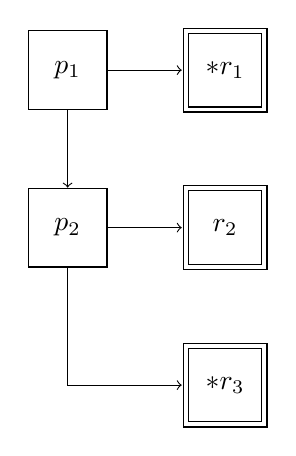
\begin{tikzpicture}[x=20mm, y=20mm]
        \tikzset{Pred/.style={shape=rectangle, draw, minimum width=1cm, minimum height=1cm}}
        \tikzset{Res/.style={shape=rectangle, draw, double distance=0.5mm, outer sep=0.5mm, minimum width=1cm, minimum height=1cm}}
        
        % nodes
        \node[Pred] (p1) at (0, 2) {$p_1$};
        \node[Res]  (r1) at (1, 2) {$\ast r_1$};
        
        \node[Pred] (p2) at (0, 1) {$p_2$};
        \node[Res] (r2) at (1, 1) {$r_2$};
        
        \node[Res] (r3) at (1, 0) {$\ast r_3$};
        
        % arrows
        \draw[->] (p1) -> (r1);
        \draw[->] (p1) -- (p2);
        \draw[->] (p2) -- (r2);
        \draw[->] (p2) |- (r3);
    \end{tikzpicture}
    \subcaption{Logical flow of a simple \CASE-expression with callsites in $r_1$ and $r_3$.}\label{flow:simple_case}
    \end{minipage}\hfill
    \begin{minipage}[b]{.45\linewidth}
    \centering 
    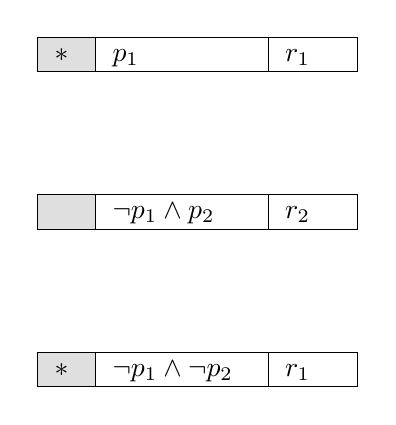
\begin{tikzpicture}[x=20mm, y=20mm]
        \node (case1) at (5, 2) {\begin{tabular}{|p{3mm}|p{5em}|p{2em}|}\hline
        \cellcolor{gray!25} $\ast$ & $p_1$ & $r_1$\\\hline
        \end{tabular}};
        
        \node (case1) at (5, 1) {\begin{tabular}{|p{3mm}|p{5em}|p{2em}|}\hline
        \cellcolor{gray!25} ~~ & $\neg p_1 \land p_2$ & $r_2$\\\hline
        \end{tabular}};
        
        \node (case1) at (5, 0) {\begin{tabular}{|p{3mm}|p{5em}|p{2em}|}\hline
        \cellcolor{gray!25} $\ast$ & $\neg p_1 \land \neg p_2$ & $r_1$\\\hline
        \end{tabular}};
    \end{tikzpicture}
    \subcaption{Generated scenarios for each branch of the \CASE-expression.}\label{scenarios:simple_case}
    \end{minipage}
    \caption{}\label{rule:base_and_rec}
\end{figure}

%\setlength{\tabcolsep}{2pt}

\subsection{Recursive \WHEN's}

Recursive predicates cannot be evaluated during callgraph creation and are therefore considered as part of the result (recursive) expression. Slicing stops \textit{before} the recursive predicate and the entire remaining \texttt{CASE}-expression is considered a single big recursive scenario.

\begin{figure}[h!]
    \centering
\begin{tikzpicture}[x=20mm, y=20mm]
\tikzset{Pred/.style={shape=rectangle, draw, minimum width=1cm, minimum height=1cm}}
\tikzset{Res/.style={shape=rectangle, draw, double distance=0.5mm, outer sep=0.5mm, minimum width=1cm, minimum height=1cm}}

% nodes
\node[Pred] (p1) at (0, 1.5) {$p_1$};
\node[Res]  (r1) at (1, 1.5) {$r_1$};
\node at (4, 1.5) {\begin{tabular}{|p{3mm}|p{5em}|p{2em}|}\hline
\cellcolor{gray!25} & $p_1$ & $r_1$\\\hline
\end{tabular}};

\node[Res, inner sep=3mm] (res) at (0.5, 0) {
    \begin{tikzpicture}[x=20mm, y=20mm, inner sep=1em]
        \node (p2) at (0, 1) {$\ast p_2$};
        \node (r2) at (1, 1) {$r_2$};
        \node (r3) at (1, 0) {$r_3$};
        \draw[->] (p2) -- (r2);
        \draw[->] (p2) |- (r3);
    \end{tikzpicture}
};
\node at (4, 0) {\begin{tabular}{|c|c|c|}\hline
\cellcolor{gray!25} $\ast$ & $\neg p_1$ & $\CASE ~ \WHEN ~p_2~ \THEN ~r_2~ \ELSE ~r_3~\END$\\\hline
\end{tabular}};
% arrows
\draw[->] (p1) -> (r1);
\draw[->] (p1) -> (0, 0.95);
\end{tikzpicture}
    \caption{Logical flow and resulting scenarios of a \texttt{CASE}-expression with a recursive predicate. Everything after and including the recursive predicate is considered one single recursive scenario.}
    \label{fig:my_label}
\end{figure}

This introduces a important constraint: No more callsites after a recursive predicate. The template for the callgraph creation makes the assumption that all callsites in a scenario must be evaluated. If the evaluation of one callsite depends on the evaluation of an other, a finally not evaluated callsite may be evaluated anyway. This can cause nontermination or runtime errors.

\subsection{Nonrecursive subtrees}
Subtrees with no callsite are taken as one big basecase. There is no need to do any further analysis because there are no more callsites that need to be seperated into their evaluation scenarios so that the callgraph can be built. In this case, the \RBASE-rule just adds the entire remaining \texttt{CASE}-expression to $B$.

\begin{figure}[h!]
    \centering
\begin{tikzpicture}[x=20mm, y=20mm]
\tikzset{Pred/.style={shape=rectangle, draw, minimum width=1cm, minimum height=1cm}}
\tikzset{Res/.style={shape=rectangle, draw, double distance=0.5mm, outer sep=0.5mm, minimum width=1cm, minimum height=1cm}}

% nodes
\node[Pred] (p1) at (0, 1.5) {$p_1$};
\node[Res]  (r1) at (1, 1.5) {$\ast r_1$};
\node at (4, 1.5) {\begin{tabular}{|p{3mm}|p{5em}|p{2em}|}\hline
\cellcolor{gray!25} $\ast$ & $p_1$ & $r_1$\\\hline
\end{tabular}};

\node[Res, inner sep=3mm] (res) at (0.5, 0) {
    \begin{tikzpicture}[x=20mm, y=20mm, inner sep=1em]
        \node (p2) at (0, 1) {$p_2$};
        \node (r2) at (1, 1) {$r_2$};
        \node (r3) at (1, 0) {$r_3$};
        \draw[->] (p2) -- (r2);
        \draw[->] (p2) |- (r3);
    \end{tikzpicture}
};
\node at (4, 0) {\begin{tabular}{|c|c|c|}\hline
\cellcolor{gray!25} ~~ & $\neg p_1$ & $\CASE ~ \WHEN ~p_2~ \THEN ~r_2~ \ELSE ~r_3~\END$\\\hline
\end{tabular}};
% arrows
\draw[->] (p1) -> (r1);
\draw[->] (p1) -> (0, 0.95);
\end{tikzpicture}
    \caption{A \texttt{CASE}-expression where no of the later branches have a callsite. Therefore the \RBASE-rule takes them all as a basecase.}
    \label{fig:case_nonrecursive}
\end{figure}


\subsection{Nested Case in \THEN}

\texttt{CASE}-expression can be nested. Nesting can happen either within the predicate of the \texttt{WHEN}-part, or within the result of \texttt{THEN}-part. As dependant callsites are forbidden, either the predicate or the result can have a nested \texttt{CASE}-expression with a callsite, but not both. If there is a nested \texttt{CASE}-expression without a callsite, it is left unchanged (\RBASE-rule).

If a \CASE-expression is located in the \texttt{THEN}-part, the inner expression is analyzed independently. The predicate from the outer scenario is prepended to the predicates of the scenarios that are generated by the inner \CASE-expression.

%Predicates must be evaluable directly for our translation template, ie. no callsite may be present in any predicate. Therefore, as soon as a predicate appears to be recursive, the recursive predicate is considered part of the recursive result and the evaluation of the \CASE-expression halts with the remaining \CASE-expression which forms an recursive case as a whole.
\begin{figure}[h!]
    \centering
    \begin{tikzpicture}[x=20mm, y=20mm]
\tikzset{Pred/.style={shape=rectangle, draw, minimum width=1cm, minimum height=1cm}}
\tikzset{Box/.style={shape=rectangle, draw, minimum width=1cm, minimum height=1cm, dotted, very thick}}
\tikzset{Res/.style={shape=rectangle, draw, double distance=0.5mm, outer sep=0.5mm, minimum width=1cm, minimum height=1cm}}

% nodes
\node[Pred] (p) at (0.5, 1) {$p$};
\node[Box]  (r1) at (2, 1) {
    \begin{tikzpicture}[x=15mm, y=15mm]
        \node[Pred] (p1) at (0, 2) {$p_1$};
        \node[Res] (r1) at (1, 2) {$r_1$};
        
        \node[Pred] (pi) at (0, 1) {$p_2$};
        \node[Res] (ri) at (1, 1) {$r_2$};
        
        \node[Res] (rn) at (1, 0) {$\ast r_3$};
        % arrows
        \draw[->] (p1) -- (r1);
        \draw[->] (pi) -- (ri);
        \draw[->] (p1) -- (pi);
        \draw[->] (pi) |- (rn);
    \end{tikzpicture}
};
\node at (5, 1.75) {
    \begin{tabular}{|p{1em}|p{2.5cm}|c|}\hline
    \cellcolor{gray!25}  & $p \land \phantom{\neg}p_1$ & $r_1$\\\hline
    \end{tabular}
};
    
\node at (5, 1) {
    \begin{tabular}{|p{1em}|p{2.5cm}|c|}\hline
    \cellcolor{gray!25}  & $p \land \neg p_1 \land \phantom{\neg} p_2$ & $r_2$\\\hline
    \end{tabular}
};

\node at (5, 0.25) {
    \begin{tabular}{|p{1em}|p{2.5cm}|c|}\hline
    \cellcolor{gray!25}$\ast$   & $p \land \neg p_1 \land \neg p_2$ & $r_3$\\\hline
    \end{tabular}
};
   
% arrows
\draw[->] (p) -- (r1);
\end{tikzpicture}
    \caption{Nested \texttt{CASE} in the predicate.}
    \label{fig:case_nested_in_when}
\end{figure}

\subsection{Nested Case in \WHEN's}
\texttt{CASE}-expression can be nested inside the \texttt{WHEN}-part of an other \texttt{CASE}-expression. Only if the inner \texttt{CASE}-expression contains a callsite, it will be analyzed.

The nested \texttt{CASE}-expression is analyzed and number of scenarios are returned. The particuliarity is here that the results of the scenarios are predicates. The scenario of the nested \texttt{CASE}-expression contains a predicate for a predicate. Therefore both, the predicate and the result of the inner scenarios, need to be added to the predicate of the outer scenario.

\begin{figure}[h!]
    \centering
\begin{tikzpicture}[x=15mm, y=12mm]
\tikzset{Pred/.style={shape=rectangle, draw, minimum width=1cm, minimum height=1cm}}
\tikzset{Box/.style={shape=rectangle, draw, minimum width=1cm, minimum height=1cm, dotted, very thick}}
\tikzset{Res/.style={shape=rectangle, draw, double distance=0.5mm, outer sep=0.5mm, minimum width=1cm, minimum height=1cm}}

% dash pattern=on 5pt off 1pt on 3pt off 3pt on 1pt off 2pt on 1pt off 2pt on 3pt off 1pt

% nodes
\node[Pred] (p) at (0, 3) {$p$};

\node[Box] (p1) at (0, 1) {
    \begin{tikzpicture}[x=15mm, y=15mm]
        \node[Pred] (p2) at (0, 1) {$\pi_1$};
        \node[Pred] (r2) at (1, 1) {$p_1$};
        \node[Pred] (p3) at (1, 0) {$\ast p_2$};
        % arrows
        \draw[->] (p2) -- (r2);
        \draw[->] (p2) |- (p3);
    \end{tikzpicture}
};
\node[Res] (r1) at (2, 1) {$r_i$};
\node (case1) at (6, 1) {
    \begin{tabular}{|p{1em}|r|c|}\hline
    \cellcolor{gray!25} & $\neg p \land \pi_1 \land \phantom{\neg} p_1$ & $r_i$\\\hline
    \cellcolor{gray!25} & $\neg p \land \pi_1 \land \neg p_1$ & $r$\\\hline
    \end{tabular}
};

\node[Res] (r) at (2, -1) {$r$};
\node (case1) at (6, -1) {
    \begin{tabular}{|p{1em}|r|c|}\hline
    \cellcolor{gray!25} $\ast$ & $\neg p \land \neg \pi_i$ & \texttt{WHEN }$p_2$ \texttt{THEN} $r_i$ \texttt{ELSE} $r$\\\hline
    \end{tabular}
};
% arrows
\draw[->] (p) -- (p1);
\draw[->] (p1) -- (r1);
\draw[->] (p1) |- (r);
\end{tikzpicture}
    \caption{Nested \texttt{CASE} in \texttt{WHEN}-part. Note that neither $r_i$ nor $r$ must contain any callsite.}
    \label{fig:case_nested_when}
\end{figure}

\subsection{\CASE- and \ELSE-rule}

The \RWHEN-rule works branch by branch. It is only applicable if not both, the predicate $p$ and the remaining branches $bs$, contain callsites (1st premise). Predicate $p$ and resulting expression $e$ are analyzed, obtaining scenarios $(B_p, R_p)$ for the predicate and $(B_e, R_e)$ for the resulting expression (2nd and 3rd premise). The nonrecursive scenarios of the predicate $B_p$ contain $n$ tuples of a predicate (of the scenario, ie. the "predicate of the predicate") and a result, the actual predicate (4th premise).

The last premise analyzes the remaining branches for those scenarios where the predicate is nonrecursive (this from $B_p$). The predicate of the remaining branches is thus prepended with the (positive) predicate of the predicate $p_p$ and the negative actual predicate $p'$. The scenarios from later branches are added below in the actual rule to set of nonrecursive resp. recursive scenarios.

\begin{figure}[h!]
    \centering\small
$$\inferrule{
    \neg (\hasCallsite(p) \land \hasCallsite(bs))\\\\
    T, C \vdash (\TRUE, p) \rightarrow (B_p, R_p) \\\\
    T, C \vdash (\TRUE, e) \rightarrow (B_e, R_e)\\\\
    B_p = \{(p_{p_1}, p'_1), ..., (p_{p_n}, p'_n)\} \\\\
    \forall 1 \leq i \leq |B_p| : T, C \vdash (p_0 ~\AND~ p_{p_i}~\AND~\NOT~ p'_i,~ \CASE~ bs ~\END) \rightarrow (B_i, R_i) \\
}{
T, C \vdash (p_0, \CASE~ \WHEN ~p ~\THEN ~e ~bs ~\END) \rightarrow \\
{\begin{tabular}{L}
         \Big( \Big\{\big(p_0 ~\AND~ p_p         ~\AND~ p' ~\AND~ p_e , e'\phantom{\CASE ~ \WHEN ~  ~ \THEN ~e ~bs~ \END}\big) ~|~~(p_p, p') \in B_p, (p_e, e') \in B_e \Big\} \cup~ (\cup_{1\leq i \leq n}B_i)~~~~,\\[2mm]
\phantom{\Big(}\Big\{\big(p_0 ~\AND~ p_p         ~\AND~ p' ~\AND~ p_e , e'\phantom{\CASE ~ \WHEN ~  ~ \THEN ~e ~bs ~\END}\big) ~|~~(p_p, p') \in B_p, (p_e, e') \in R_e \Big\} \cup~ (\cup_{1\leq i \leq n}R_i) ~\cup\\
\phantom{\Big(}\Big\{\big(p_0 ~\AND~ p_p\phantom{~\AND~ p' ~\AND~ p_e},            \CASE ~ \WHEN ~p'~ \THEN ~e ~bs ~\END \big) ~|~~(p_p, p') \in R_p~~~~~~~~~~~~~~~~~  \Big\}~~~~~~~~~~~~~~~~~~~~~~~~~ \Big)
\end{tabular}}
}\quad(\textsc{when})$$
    \caption{\RWHEN-rule to slice \texttt{CASE}-expressions into its different evaluation scenarios.}
    \label{fig:my_label}
\end{figure}

The actual rule combines all sources of scenarios. The basecase scenarios (first component of the tuple) are build by combining all nonrecursive predicates ($B_p$) with the nonrecursive resulting expressions ($B_e$). These set of scenarios is unioned with the $n$ sets of scenarios from other branches $(B_i, R_i)$ (remember that $n$ is the number of nonrecursive predicate-scenarios).

The same happens analogiously for the second component of the tuple, the recursive scenarios. This time nonrecursive predicate-scenarios ($B_p$) are combined with recursive resulting expression scenarios ($B_e$). Additionally, scenarios with recursive predicates ($R_p$) are added.

When all branches are processed, a single \texttt{ELSE} remains. This is not valid SQL, therefore the \RBASE-rule has a premise that restricts applicability here. Thus we need the \RELSE-rule that takes care of unwrapping the result of this trivial conditional.
\begin{figure}[h!]
    \centering\small
$$\inferrule{
    T, C \vdash (p, e) \rightarrow (B, R) \\
}{
    T, C \vdash (p, \CASE ~\ELSE ~e~ \END) \rightarrow (B, R)
}
\quad(\textsc{else})$$
    \caption{\RELSE-rule.}
    \label{fig:my_label}
\end{figure}

With the four rules from the previous section, very simple \texttt{CASE}-expressions (with only constants or callsites) can be analyzed. Nonrecursive subtrees of the AST are handlded by the \RBASE-rule and allsites are considered with the \RREC-rule. What follows now, is a rule to traverse expressions like \texttt{1 + fn(...)}.

\section{Handling recursive operands}

\begin{wrapfigure}{r}{.3\textwidth}
  \centering
  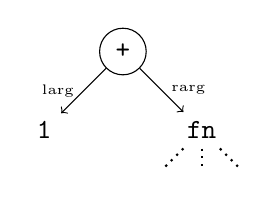
\begin{tikzpicture}
  \node[draw, circle] (plus) at (1,1) {\texttt{+}};
  \node (one) at (0,0) {\texttt{1}};
  \node (fn) at (2,0) {\texttt{fn}};
  \draw[->] (plus) to node[pos=0.5, left, label distance=5mm]{\tiny{larg}} (one);
  \draw[->] (plus) to node[pos=0.5, right, label distance=5mm]{\tiny{rarg}} (fn);
  \draw[dotted, thick] (fn) to +(-0.5, -0.5);
  \draw[dotted, thick] (fn) to +(0, -0.5);
  \draw[dotted, thick] (fn) to +(0.5, -0.5);
  \end{tikzpicture}
  \caption{AST-representation of \texttt{1 + fn(...)}.}
  \label{ast:expr}
\end{wrapfigure}

Expressions like \texttt{1 + fn(...)} cannot be translated by the \RBASE-rule nor by the \RREC-rule because the the callsite is not at the root of the AST, it is located of one of its subtrees. At the root, there is the \texttt{+}-operator, the left subtree is the constant \texttt{1} and the right subtree the callsite \texttt{fn(...)} (\autoref{ast:expr}).

The \REXPR-rules purpose is to traverse the AST and to analyze each subtree independently. I use the generic term of a \textit{function} to refer to syntactic constructs that consists of a node with multiple subtrees that are independent from each other. Beside built-in functions and UDFs those are operators, aggregates, subquery expressions (eg. \texttt{n IN (...)}), row-comparisons, array-element access, arrays itself and \texttt{VALUES}-lists. The last may surprising first, but \texttt{(VALUES (1), (2), (3))} or \texttt{ARRAY[1, 2, 3]} is nothing else than a constructor -- a function.

\begin{figure}[h]
    \centering
    \footnotesize
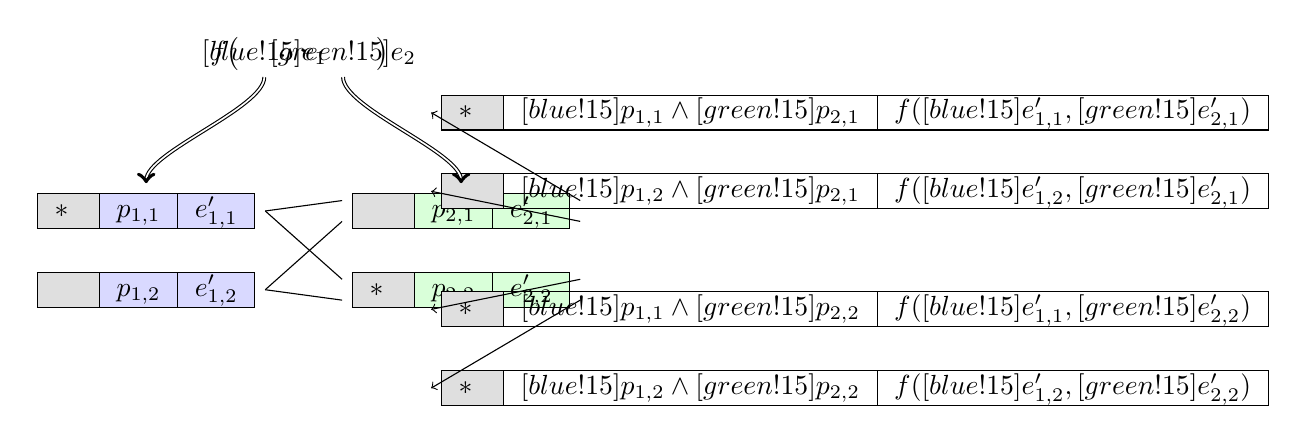
\begin{tikzpicture}[x=10mm, y=10mm]
\node      at (1, 5) {$f\big($};
\node (e1) at (1.5, 5) {$\highlight[blue!15]{e_1}$};
\node      at (2, 5) {$,$};
\node (e2) at (2.5, 5) {$\highlight[green!15]{e_2}$};
\node      at (3, 5) {$\big)$};

\node (e11) at (0, 3) { 
    \begin{tabular}{|p{1em}|r|c|}\hline
    \cellcolor{gray!25} $\ast$ & \cellcolor{blue!15}${p_{1,1}}$ & \cellcolor{blue!15}${e'_{1,1}}$\\\hline
    \end{tabular}
};
\node (e12) at (0, 2) { 
    \begin{tabular}{|p{1em}|r|c|}\hline
    \cellcolor{gray!25}  & \cellcolor{blue!15}${p_{1,2}}$ & \cellcolor{blue!15}${e'_{1,2}}$\\\hline
    \end{tabular}
};

\node (e21) at (4, 3) { 
    \begin{tabular}{|p{1em}|r|c|}\hline
    \cellcolor{gray!25}  & \cellcolor{green!15}${p_{2,1}}$ & \cellcolor{green!15}${e'_{2,1}}$\\\hline
    \end{tabular}
};
\node (e22) at (4, 2) { 
    \begin{tabular}{|p{1em}|r|c|}\hline
    \cellcolor{gray!25}$\ast$ & \cellcolor{green!15}${p_{2,2}}$ & \cellcolor{green!15}${e'_{2,2}}$\\\hline
    \end{tabular}
};

\node (r1) at (9, 4.25) { 
    \begin{tabular}{|p{1em}|r|c|}\hline
    \cellcolor{gray!25} $\ast$ & $\highlight[blue!15]{p_{1,1}} \land \highlight[green!15]{p_{2,1}}$ & $f(\highlight[blue!15]{e'_{1,1}}, \highlight[green!15]{e'_{2,1}})$\\\hline
    \end{tabular}
};
\node (r2) at (9, 3.25) { 
    \begin{tabular}{|p{1em}|r|c|}\hline
    \cellcolor{gray!25}  & $\highlight[blue!15]{p_{1,2}} \land \highlight[green!15]{p_{2,1}}$ & $f(\highlight[blue!15]{e'_{1,2}}, \highlight[green!15]{e'_{2,1}})$\\\hline
    \end{tabular}
};

\node (r3) at (9, 1.75) { 
    \begin{tabular}{|p{1em}|r|c|}\hline
    \cellcolor{gray!25} $\ast$ & $\highlight[blue!15]{p_{1,1}} \land \highlight[green!15]{p_{2,2}}$ & $f(\highlight[blue!15]{e'_{1,1}}, \highlight[green!15]{e'_{2,2}})$\\\hline
    \end{tabular}
};
\node (r4) at (9, 0.75) { 
    \begin{tabular}{|p{1em}|r|c|}\hline
    \cellcolor{gray!25} $\ast$ & $\highlight[blue!15]{p_{1,2}} \land \highlight[green!15]{p_{2,2}}$ & $f(\highlight[blue!15]{e'_{1,2}}, \highlight[green!15]{e'_{2,2}})$\\\hline
    \end{tabular}
};
\draw[->, double, out=270, in=90, looseness = 0.5] (e1.south) to (e11);
\draw[->, double, out=270, in=90, looseness = 0.5] (e2.south) to (e21);

\draw (e11.east) -- (e21.175);
\draw (e11.east) -- (e22.175);
\draw (e12.east) -- (e21.185);
\draw (e12.east) -- (e22.185);

\draw[->] (e21.5) -- (r1.west);
\draw[->] (e21.355) -- (r2.west);
\draw[->] (e22.5) -- (r3.west);
\draw[->] (e22.355) -- (r4.west);
\end{tikzpicture}

    \caption{Operands of a function are translated separately. For each operand a number of scenarios is generated. All possible scenarios of the original function are created by using the cross product.}
    \label{fig:expr-expr}
\end{figure}

Multiple evaluation scenarios may be obtained for each subtree. These scenarios need to be combined again to return the different evaluation scenarios of the function itself. This is done by building the cross product between the scenarios of each subtree. We obtain all possible combinations of evaluation scenarios of the subtrees, constituting the scenarios of the function (\autoref{fig:expr-expr}).

\iffalse
$
\inferrule*[Right=(expr)]{
    \inferrule*[Left=(rec)]{ }{
        {\begin{minipage}[b]{15em}
        \mintinline{postgresql}{(TRUE, fib($1 - 1)) ->}
        \mintinline{postgresql}{({}, {(TRUE, fib($1 - 1))})}
        \end{minipage}}
    }\\
    \inferrule*[Right=(rec)]{ }{
        {\begin{minipage}[b]{15em}
        \mintinline{postgresql}{(TRUE, fib($1 - 2)) ->}
        \mintinline{postgresql}{({}, {(TRUE, fib($1 - 2))})}
        \end{minipage}}
    }
}{
    {\begin{minipage}[b]{25em}
    \mintinline{postgresql}{(TRUE, fib($1 - 1) + fib($1 - 2)) ->}
    \mintinline{postgresql}{({}, {(TRUE AND TRUE AND TRUE, fib($1 - 1) + fib($1 - 2))})}
    \end{minipage}}
}
$
\fi

The \REXPR formalizes this pattern. As meta-variable for any suitable function etc. $\oplus$ is used. Each subtree $e_i$ is translated independently, resulting in the $1 \leq i \leq n$ tuples of scenarios $(B_i, R_i$). Note that the rule is only applicable if at least on subtree contains a callsite, otherwise it would overlap with \RBASE.

Nonrecursive scenarios of the function are created by replacing each argument with the expression from one of its scenarios. The cross product between all nonrecursive scenarios $B_i$ is used to build a set of all possible combinations of nonrecursive scenarios. The predicates $p_i$ of the scenario of each of the $n$ arguments are all unioned by \texttt{AND}. The arguments of the original function is replaced with the expressions generated by the scenarios.

To create all scenarios of the function where at least one argument is recursive, the cross product between all scenarios of an argument (recursive and nonrecursive) is built. Only those combinations where at least one expression is recursive are kept.

$$\quad(\textsc{expr})\inferrule{
    \exists i \in \{1, ..., n\}: T \vdash \hasCallsite(e_i)\\
    \forall i \in \{1, ..., n\}: T, C \vdash (\TRUE, e_i) \rightarrow (B_i, R_i)
}{
    T, C \vdash (p, \oplus_{1\leq i \leq n} e_i) \rightarrow \\\\
    {\begin{tabular}[b]{LLL}
        (&\{(p ~\AND~ (\AND_{1\leq i \leq n} p_i)), \oplus_{1\leq i \leq n} e_i' &~|~~ ((p_1, e_1'), ..., (p_n, e_n')) \in \times_{\{i|1\leq i \leq n\}} ~B_i\}, \\
        &\{(p ~\AND~ (\AND_{1\leq i \leq n } p_i)), \oplus_{1\leq i \leq n} e_i &~|~~ ((p_1, e_1'), ..., (p_n, e_n')) \in \times_{\{i|1\leq i \leq n\}} (B_i \cup R_i),\\&&~~~~\exists e \in \{e'_1, ..., e'_n\} : \hasCallsite(T, e)\})
    \end{tabular}}
}$$


\begin{figure}
    \centering
    {\small
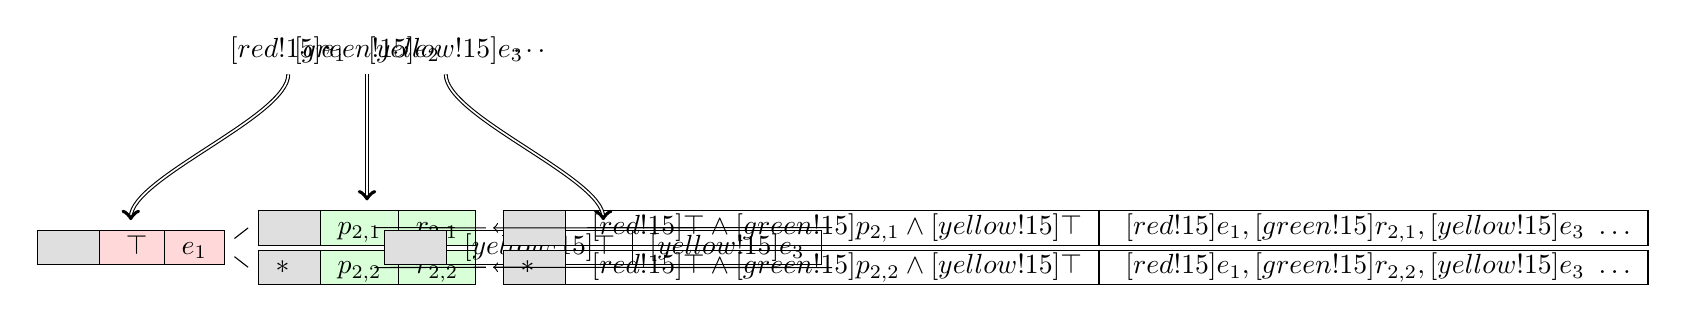
\begin{tikzpicture}[x=5mm, y=5mm]
\node      at ( 8, 9) {$\SELECT$};
\node (e1) at (10, 9) {$\highlight[red!15]{e_1}$};
\node      at (11, 9) {$,$};
\node (e2) at (12, 9) {$\highlight[green!15]{e_2}$};
\node      at (13, 9) {$,$};
\node (e3) at (14, 9) {$\highlight[yellow!15]{e_3}$};
\node      at (16, 9) {$\FROM ~ \dots$};

\node (e11) at (6, 4) { 
    \begin{tabular}{|p{1em}|r|c|}\hline
    \cellcolor{gray!25}  & \cellcolor{red!15} $\top$ & \cellcolor{red!15}$e_1$\\\hline
    \end{tabular}
};

\node (e21) at (12, 4.5) { 
    \begin{tabular}{|p{1em}|r|c|}\hline
    \cellcolor{gray!25}  & \cellcolor{green!15}$p_{2,1}$ & \cellcolor{green!15}$r_{2,1}$\\\hline
    \end{tabular}
};
\node (e22) at (12, 3.5) { 
    \begin{tabular}{|p{1em}|r|c|}\hline
    \cellcolor{gray!25} $\ast$ & \cellcolor{green!15}$p_{2,2}$ & \cellcolor{green!15}$r_{2,2}$\\\hline
    \end{tabular}
};

\node (e31) at (18, 4) { 
    \begin{tabular}{|p{1em}|r|c|}\hline
    \cellcolor{gray!25} & $\highlight[yellow!15]{\top}$ & $\highlight[yellow!15]{e_3}$\\\hline
    \end{tabular}
};

\node (r1) at (30, 4.5) { 
    \begin{tabular}{|p{1em}|r|c|}\hline
    \cellcolor{gray!25}  & $\SELECT ~ \highlight[red!15]{\top} \land \highlight[green!15]{p_{2,1}} \land \highlight[yellow!15]{\top}$ & $\SELECT~ \highlight[red!15]{e_1}, \highlight[green!15]{r_{2,1}}, \highlight[yellow!15]{e_3} ~ \FROM \dots$\\\hline
    \end{tabular}
};
\node (r2) at (30, 3.5) { 
    \begin{tabular}{|p{1em}|r|c|}\hline
    \cellcolor{gray!25} $\ast$ & $\SELECT ~ \highlight[red!15]{\top} \land \highlight[green!15]{p_{2,2}} \land \highlight[yellow!15]{\top}$ & $\SELECT~ \highlight[red!15]{e_1}, \highlight[green!15]{r_{2,2}}, \highlight[yellow!15]{e_3} ~ \FROM \dots$\\\hline
    \end{tabular}
};
\draw[->, double, out=270, in=90, looseness = 0.5] (e1.south) to (e11);
\draw[->, double, out=270, in=90, looseness = 0.5] (e2.south) to (e21);
\draw[->, double, out=270, in=90, looseness = 0.5] (e3.south) to (e31);
\draw (e11.5) to (e21.west);
\draw (e11.355) to (e22.west);
\draw (e21.east) to (e31.175);
\draw (e22.east) to (e31.185);
\draw[->] (e31.5) -- (r1.west);
\draw[->] (e31.355) -- (r2.west);
%\draw[->, bend left=20]  (e11.north) to (e21.north) to (e31.north) to (r1.west);
%\draw[->, bend right=20] (e11.south) to (e22.south) to (e31.south) to (r2.west);
\end{tikzpicture}}
    \caption{The projection of a relation happening inside \SELECT~can be understood as a function $\SELECT(e_1, \dots, e_n, T)$. The same happens analogously for the \FROM-clause: $\FROM(T_1, \dots, T_m)$}
    \label{fig:expr-select}
\end{figure}

\begin{figure}
    \centering
    {\small
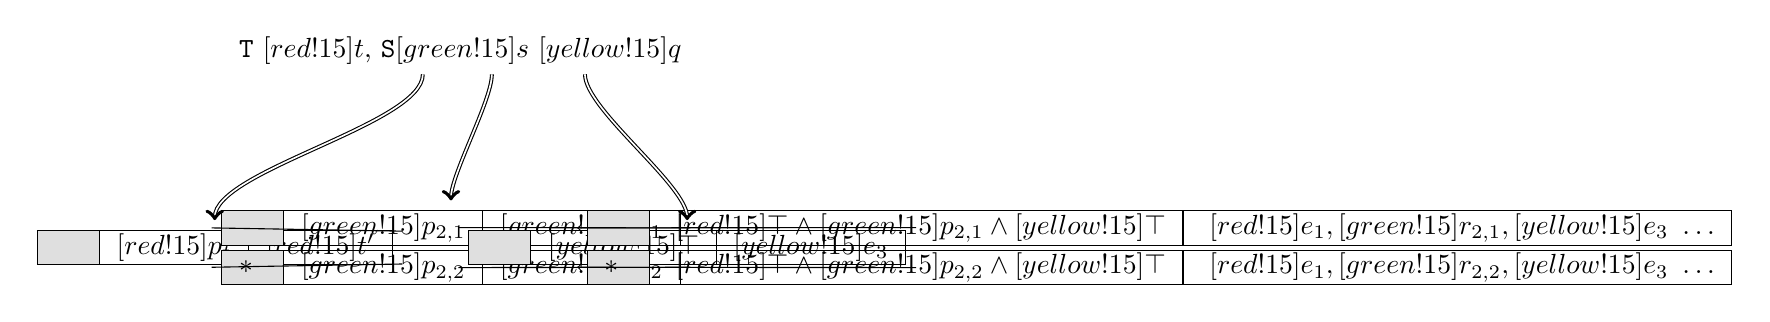
\begin{tikzpicture}[x=5mm, y=5mm, node distance=1mm]
\node (ctes) at (12,9) {\WITH~ \texttt{T} \AS $\highlight[red!15]{t}$, \texttt{S}\AS $\highlight[green!15]{s}$ $\highlight[yellow!15]{q}$};

\node (e11) at (6, 4) { 
    \begin{tabular}{|p{1em}|r|c|}\hline
    \cellcolor{gray!25}  & $\highlight[red!15]{p_t}$ & $\highlight[red!15]{t'}$\\\hline
    \end{tabular}
};

\node (e21) at (12, 4.5) { 
    \begin{tabular}{|p{1em}|r|c|}\hline
    \cellcolor{gray!25}  & $\highlight[green!15]{p_{2,1}}$ & $\highlight[green!15]{r_{2,1}}$\\\hline
    \end{tabular}
};
\node (e22) at (12, 3.5) { 
    \begin{tabular}{|p{1em}|r|c|}\hline
    \cellcolor{gray!25} $\ast$ & $\highlight[green!15]{p_{2,2}}$ & $\highlight[green!15]{r_{2,2}}$\\\hline
    \end{tabular}
};

\node (e31) at (18, 4) { 
    \begin{tabular}{|p{1em}|r|c|}\hline
    \cellcolor{gray!25} & $\highlight[yellow!15]{\top}$ & $\highlight[yellow!15]{e_3}$\\\hline
    \end{tabular}
};

\node (r1) at (30, 4.5) { 
    \begin{tabular}{|p{1em}|r|c|}\hline
    \cellcolor{gray!25}  & $\SELECT ~ \highlight[red!15]{\top} \land \highlight[green!15]{p_{2,1}} \land \highlight[yellow!15]{\top}$ & $\SELECT~ \highlight[red!15]{e_1}, \highlight[green!15]{r_{2,1}}, \highlight[yellow!15]{e_3} ~ \FROM \dots$\\\hline
    \end{tabular}
};
\node (r2) at (30, 3.5) { 
    \begin{tabular}{|p{1em}|r|c|}\hline
    \cellcolor{gray!25} $\ast$ & $\SELECT ~ \highlight[red!15]{\top} \land \highlight[green!15]{p_{2,2}} \land \highlight[yellow!15]{\top}$ & $\SELECT~ \highlight[red!15]{e_1}, \highlight[green!15]{r_{2,2}}, \highlight[yellow!15]{e_3} ~ \FROM \dots$\\\hline
    \end{tabular}
};
\draw[->, double, out=270, in=90, looseness = 0.5] (ctes.220) to (e11);
\draw[->, double, out=270, in=90, looseness = 0.5] (ctes.330) to (e21);
\draw[->, double, out=270, in=90, looseness = 0.5] (ctes.350) to (e31);
\draw (e11.5) to (e21.west);
\draw (e11.355) to (e22.west);
\draw (e21.east) to (e31.175);
\draw (e22.east) to (e31.185);
\draw[->] (e31.5) -- (r1.west);
\draw[->] (e31.355) -- (r2.west);
%\draw[->, bend left=20]  (e11.north) to (e21.north) to (e31.north) to (r1.west);
%\draw[->, bend right=20] (e11.south) to (e22.south) to (e31.south) to (r2.west);
\end{tikzpicture}}
    \caption{The ~\WITH-clause could also be viewed as composition of functions $\WITH(t, T, q)$ that binds a table-variable \texttt{T} to an expression \texttt{t} for a given query \texttt{q}. In this example it would be $\WITH(T, t, \WITH(S, s, q))$ as CTEs can reference preceding ones.}
    \label{fig:expr-cte}
\end{figure}

If the callsites of a query a located in the \FROM-part, it means that at least one table referenced is recursive, ie. contains a callsite or a reference a recursive table. 
As the tables within the same \FROM cannot reference each other, we can process each table independently and resemble the whole query with all possible combinations, similar to the \REXPR-rule. For an example see this example:
\sqlcode[mathescape=true]{snippets/rule_from_example.sql}


$
\inferrule*{
    \inferrule*{...}{
{\begin{minipage}[b]{12em}
\sqlcode{snippets/rules/fib/01-case.sql}
\end{minipage}}
    }
}{
{\begin{minipage}[b]{12em}
\sqlcode{snippets/rules/fib/01-select.sql}
\end{minipage}}
}
$


$$\quad(\textsc{select})\inferrule{
    \exists i \in \{1, ..., k\}: T \vdash \hasCallsite(e_{s_i}) \\
    \forall i \in \{1 \leq i \leq n\} : T \vdash \neg \hasCallsite(e_{t_i}) \\
    T \vdash \neg \hasCallsite(e_{w}) \\
    \forall i \in \{1, ..., k\}: T, \varnothing \vdash (\TRUE, e_{s_i}) \rightarrow (B_i, R_i)
}{
    T, \varnothing \vdash (p, \SELECT [\texttt{DISTINCT}]~ e_{s_1}, ..., e_{s_k} \FROM t_1 \AS a_1 \otimes ... \otimes  t_n \AS a_n \WHERE e_w) \rightarrow \\\\
    {\begin{tabular}[b]{LLLL}
    (~~&\{&(&\SELECT p ~\AND~ p_{s_1} ~\AND~ \cdots ~\AND~ p_{s_k},\\
        &&&\SELECT [\texttt{DISTINCT}]~ e'_{s_1}, ..., e'_{s_k} \FROM t_1 \AS a_1 \otimes ... \otimes  t_n \AS a_n \WHERE e_w~~) \\
        && | &~((p_{s_1}, e'_{s_1}), ..., (p_{s_k}, e'_{s_k})) \in \times_{1 \leq i \leq k} B_i~~\}, \\
     &\{&(&\SELECT p ~\AND~ p_{s_1} ~\AND~ \cdots ~\AND~ p_{s_k}, \\
        &&&\SELECT [\texttt{DISTINCT}]~ e'_{s_1}, ..., e'_{s_k} \FROM t_1 \AS a_1 \otimes ... \otimes  t_n \AS a_n \WHERE e_w~~) \\
        && | &~((p_{s_1}, e'_{s_1}), ..., (p_{s_k}, e'_{s_k})) \in \times_{1 \leq i \leq k} (B_i \cup R_i), \exists e \in \{e'_{s_1}, ..., e'_{s_k}\} : \hasCallsite(e)~~\}~~)\\
    \end{tabular}}
}$$
\subsection{WHERE-Rule}
$$\quad(\textsc{where})\inferrule{
    T \vdash \neg \hasCallsite(e_{s}) \\
    \forall i \in \{1 \leq i \leq n\} : T \vdash \neg \hasCallsite(e_{t_i}) \\
    T \vdash \hasCallsite(e_{w}) \\
    T, \varnothing \vdash (p, e_{w}) \rightarrow (B, R)
}{
    T, \varnothing \vdash (p, \SELECT e_s \FROM t_1 \AS a_1 \otimes ... \otimes  t_n \AS a_n \WHERE e_w) \rightarrow \\\\
    {\begin{tabular}[b]{LLLL}
    (~~&\{&(&\SELECT p_w  \FROM t_1 \AS a_1 \otimes ... \otimes  t_n \AS a_n \WHERE e'_w,\\
        &&&\SELECT e_s \FROM t_1 \AS a_1 \otimes ... \otimes  t_n \AS a_n \WHERE e'_w~~) \\
        && | &~(p_w, e'_w) \in B~~\}, \\
     &\{&(&\SELECT p_w \FROM t_1 \AS a_1 \otimes ... \otimes  t_n \AS a_n \WHERE e'_w, \\
        &&&\SELECT e_s \FROM t_1 \AS a_1 \otimes ... \otimes  t_n \AS a_n \WHERE e'_w~~) \\
        && | &~(p_w, e'_w) \in R~~\}~~)\\
    \end{tabular}}
}$$
\\
\section{Handling CTEs}
% Without CTEs hasCallsite just checks the subtree
The notion of \textit{containing a callsite} (or being \textit{recursive}) is simple when considering only S-F-W queries. If a SQL-fragment $e$ contains a callsite, the subexpression is recursive: $\hasCallsite(e) = fn \sqsubset e$. From an implementation point of view, it is as simple as filtering the AST of $e$ for callsites.

(\autoref{fig:trimmed_ref}), (\autoref{fig:simple_indiref})

\begin{wrapfigure}{r}{.5\textwidth}\vspace{-5mm} 
    \begin{minipage}{\linewidth}
    \label{fig:simple_indiref}\par\vfill
    \begin{minted}{sql}
    WITH S AS (SELECT f(n-1)),
         T AS (SELECT * FROM S)
    SELECT * FROM T
    \end{minted}
    \subcaption{Neither the actual query nor the referenced CTE \texttt{T} directly contains a callsite.}
    \label{fib_nonrec_scenarios}\par\vfill
    \begin{minted}{sql}
    SELECT (
        WITH T AS (SELECT f(n-1))
        SELECT 1
    )
    \end{minted}
    \subcaption{Our definition of $\hasCallsite$ would fail here since a callsite is located in the subtree. The query is acutally nonrecursive.}
    \label{fig:trimmed_ref}
\end{minipage}
\caption{}
\label{lst:indirect_callsite_ref}\vspace{-5mm} 
\end{wrapfigure}

% CTEs introduce indirect callsites that make callsite detection more complicated
With CTEs we need to take into account two things. First, callsites can now be located outside the current subtree by referencing recursive CTEs. Second, a scenario may contain unused recursive CTEs, fooling $\hasCallsite$ as stated above to believe a given SQL-fragment is recursive, even if the recursive CTEs are unused and thus never evaluated.

% Removing all CTEs, translating then and then reattaching only used CTEs fixes this.
We can take this issues into account, if we remove the CTEs from the original query before translating the actual query. For each query-scenario only those CTEs are reattached afterwards, that are actually used (\autoref{tracking_recursive_ctes}). To detect indirect callsite references, we note recursive CTEs when detaching (\autoref{tracking_cte_dependencies}) and check against that list if we encounter free table-variables in the query.

\subsection{Tracking recursive CTEs}\label{tracking_recursive_ctes}

% Recursive CTEs are gathered step by step 
CTEs may contain callsites and therefore need to be analyzed and sliced into evaluation scenarios. They need to be processed step by step before the actual query to match the natural SQL evaluation order. If a CTE-scenario contains a callsite, its alias is added to the list of recursive CTEs $T$ in scope. Otherwise, the alias is removed from that list to take shadowing into account as CTEs can be nested (\autoref{lst:indirect_callsite_ref}). As we continue with the following CTEs, any CTE that has no direct callsite but contains a reference to a CTE in $T$ is also added itself to $T$ as the evaluation of that CTE will eventually lead to a recursive call. This way, we can build up $T$ incrementally and do not need to track each reference recursively back to its declaration to find out whether its recursive. For an example see \autoref{fig:tracking_recursive_ctes}

\begin{figure}[h]
    \small
    \centering
    \begin{tikzpicture}[x=8mm, y=8mm]
    \node at (0.5, 1) {\footnotesize{(a)}};
    \node at (5.5, 1) {\footnotesize{(b)}};
    \node at (15.5, 1) {\footnotesize{(c)}};
    \node[anchor=west] at (-1, 0) {\WITH};
    \node[anchor=west] (A) at (0, 0)  {\texttt{A} \AS $(\ast a),$};
    \node[anchor=west] (B) at (0, -1) {\texttt{B} \AS $(b),$};
    \node[anchor=west] (C) at (0, -2) {\texttt{C} \AS $(c),$};
    \node[anchor=west] (D) at (0, -3) {\texttt{D} \AS $(d)$};
    \node[anchor=north west] (S) at (-1, -3.75) {$\underbrace{\SELECT~\texttt{*}~\FROM~\texttt{D}}_q$};
    \node[anchor=west] (Ar) at (3, 0)  {$fn \sqsubset a  \Longrightarrow  \hasCallsite(T, q)$};
    \node[anchor=west] (Br) at (3, -1) {$\FV(b) \cap T = \emptyset \cap \{\texttt{A}\} = \emptyset  \Longrightarrow  \neg \hasCallsite(T, q)$};
    \node[anchor=west] (Cr) at (3, -2) {$\FV(c) \cap T = \{A\} \cap \{A\} \neq \emptyset  \Longrightarrow  \hasCallsite(T, q)$};
    \node[anchor=west] (Dr) at (3, -3) {$\FV(d) \cap T = \{C\} \cap \{A, C\} \neq \emptyset  \Longrightarrow  \hasCallsite(T, q)$};
    \node[anchor=north west] (Dr) at (3, -3.75) {$\FV(q) \cap T = \{D\} \cap \{A, C, D\} \neq \emptyset  \Longrightarrow  \hasCallsite(T, q)$};
    \node[anchor=west] (Ar) at (13.5, 0) {$T := T \cup \{\texttt{A}\} = \{\texttt{A}\}$};
    \node[anchor=west] (Br) at (13.5, -1) {$T := T \setminus \{\texttt{B}\} = \{\texttt{A}\}$};
    \node[anchor=west] (Cr) at (13.5, -2) {$T := T \cup \{\texttt{C}\} = \{\texttt{A}, \texttt{C}\}$};
    \node[anchor=west] (Dr) at (13.5, -3) {$T := T \cup \{\texttt{D}\}= \{\texttt{A}, \texttt{C}, \texttt{D}\}$};
    \draw[->, bend right=60] (C) to (A);
    \draw[->] (C) to (B);
    \draw[->] (D) to (C);
    \end{tikzpicture}
    \caption{a) $q$ has no direct callsite, but reference \texttt{D} that contains a reference to \texttt{A} via \texttt{C}. \texttt{A} contains a direct callsite. b) A fragment $e$ is considered recursive if it contains a direct callsite ($fn \sqsubset$ e) or uses a recursive table-variable. c) If $\hasCallsite$ yields true for a CTE-body, its alias is added to the set of recursive table-variables $T$. Otherwise, the alias is removed to take into account shadowing.}
    \label{fig:tracking_recursive_ctes}
\end{figure}

% Referenced CTEs are detected via unbound variables
References to CTEs can be easily extracted from a SQL-fragment by collecting unbound table-variables. Let us call the function that computes all free table-variables of a SQL-fragment $e$ $\FV(e)$. It is implemented straight forward: Each CTE definition within a \WITH-block adds its alias to the list of bound table-variables. Every reference to a table-variable that is not contained in that list is considered free.


\begin{wrapfigure}{r}{0.4\textwidth}
    \begin{minted}{sql}
    WITH T AS (SELECT fn(n-1))
    SELECT *
    FROM (
      WITH T AS (SELECT 1)
      SELECT * FROM T
    ) T
    \end{minted}
    \caption{The outer, recursive CTE \texttt{T} is shadowed by an inner CTE.}
    \label{lst:indirect_callsite_ref}
\end{wrapfigure}

% Row-references vs. table-variables
Note that there can occur two different types of free variables inside a SQL-fragment: \textit{Table-Variables} and \textit{Row-References}. Table-variables like \texttt{T} can exclusively be used in ~\FROM~ and reference an entire table. This table-variables are introduced either by the existence of a table in the current database or by an CTE. Row-references like \texttt{T.v} point to a single table-row of a table referenced by ~\FROM. Not the actual "use" of a table-variable via a row-reference causes the recursive call, but its bare existence in the FROM-clause since it is evaluated first. For this reason it is sufficient to track only \textit{table}-variables and ignore row-references entirely.

The function to judge whether a SQL-fragment is recursive looks now as follows:
\begin{align*}
    \hasCallsite(T, e) =& fn(\dots) \sqsubset e \lor \FV(e) \cap T \neq \emptyset
\end{align*}
Either the callsite is directly contained in $e$, or it has a free table-variable that is also enlisted in $T$. Otherwise the snippet is not recursive.

%We process CTEs of a \WITH-block top down, before translating the actual \SELECT-query, resembling the way SQL evaluates them. If a CTE \texttt{T} references a CTE \texttt{S} that is recursive, \texttt{T} is also recursive. SQL evaluates CTEs in the order they are defined, so that preceding CTEs can be referenced by following CTEs (figure 4.4a FIXME?). Furthermore, CTEs can be nested so that we need to take care of shadowing out outer CTEs.

%Instead of tracing every reference through the entire query until the initial definition is found, I take an incremental approach: If a new table-variable is created, we check each free variable in its subtree against the environment of known recursive table-references within that scope. If there is a recursive table referenced or the subtree contains an immediate recursive call, the new table-reference is entailed the set of recursive table-references.

%Each CTE-scenario is augmented with its dependencies to previously defined CTEs. Each CTE is sliced into its different scenarios, then each scenario is analyzed, removed from the query and stored in the queue. When all CTEs are processed and the actual query is translated, only those CTEs are reattached to the query-scenario that are actually used. Indirect callsites can be detected by simply checking if there exists a free table-variable that is enlisted in $T$.

\subsection{Tracking CTE-dependencies}\label{tracking_cte_dependencies}
As we have seen, CTEs may use other CTEs so that we need to keep track of the CTE dependencies of a query. This happens similar to the creation of the set $T$ of recursive CTEs. For each CTE \texttt{C} we collect all CTE-references \texttt{$C_i$} and add them to the set of dependencies $D_c$. Because the used CTEs may have again dependencies, they are also added to $D_c$. Because of the strict ordering we can do this step by step. See \autoref{fig:cte_deps} for an illustration.

$$\refs(q) := \FV(q) \cup \left(\bigcup_{c \in \FV(q)} \refs(c)\right)$$

\begin{figure}[h!]
    \centering
    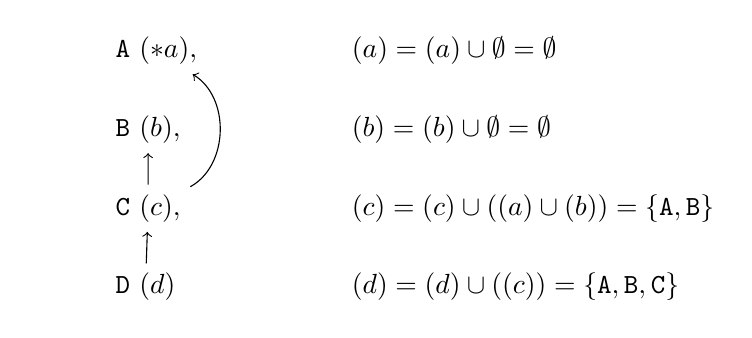
\begin{tikzpicture}[x=10mm, y=10mm]
    \node[anchor=west] at (-1, 0) {\WITH};
    \node[anchor=west] (A) at (0, 0)  {\texttt{A} \AS $(\ast a),$};
    \node[anchor=west] (B) at (0, -1) {\texttt{B} \AS $(b),$};
    \node[anchor=west] (C) at (0, -2) {\texttt{C} \AS $(c),$};
    \node[anchor=west] (D) at (0, -3) {\texttt{D} \AS $(d)$};
    \node[anchor=west] (Ar) at (3, 0)  {$\refs(a) = \FV(a) \cup \emptyset = \emptyset$};
    \node[anchor=west] (Br) at (3, -1) {$\refs(b) = \FV(b) \cup \emptyset = \emptyset$};
    \node[anchor=west] (Cr) at (3, -2) {$\refs(c) = \FV(c) \cup (\refs(a) \cup \refs(b)) = \{\texttt{A}, \texttt{B}\}$};
    \node[anchor=west] (Dr) at (3, -3) {$\refs(d) = \FV(d) \cup (\refs(c)) = \{\texttt{A}, \texttt{B}, \texttt{C}\}$};
    \draw[->, bend right=60] (C) to (A);
    \draw[->] (C) to (B);
    \draw[->] (D) to (C);
    \end{tikzpicture}
    \caption{References are tracked incrementally by collecting free table-variables (ie. direct CTE references) along with the references of those free table-variables.}
    \label{fig:cte_deps}
\end{figure}

While shadowing was an issue when tracking recursive CTEs, it does not hit us here. The difference is that the list of recurisve table-variables $T$ was passed to further computation steps while $C$ is only nonempty at the level of the current query. Any new CTE in a subexpression $e$ binds the previously free table-variable, preventing it from occurring in the CTE-dependencies. Thus, $\FV(e)$ already takes care of shadowing here.

\begin{figure}[h!]
    \centering
    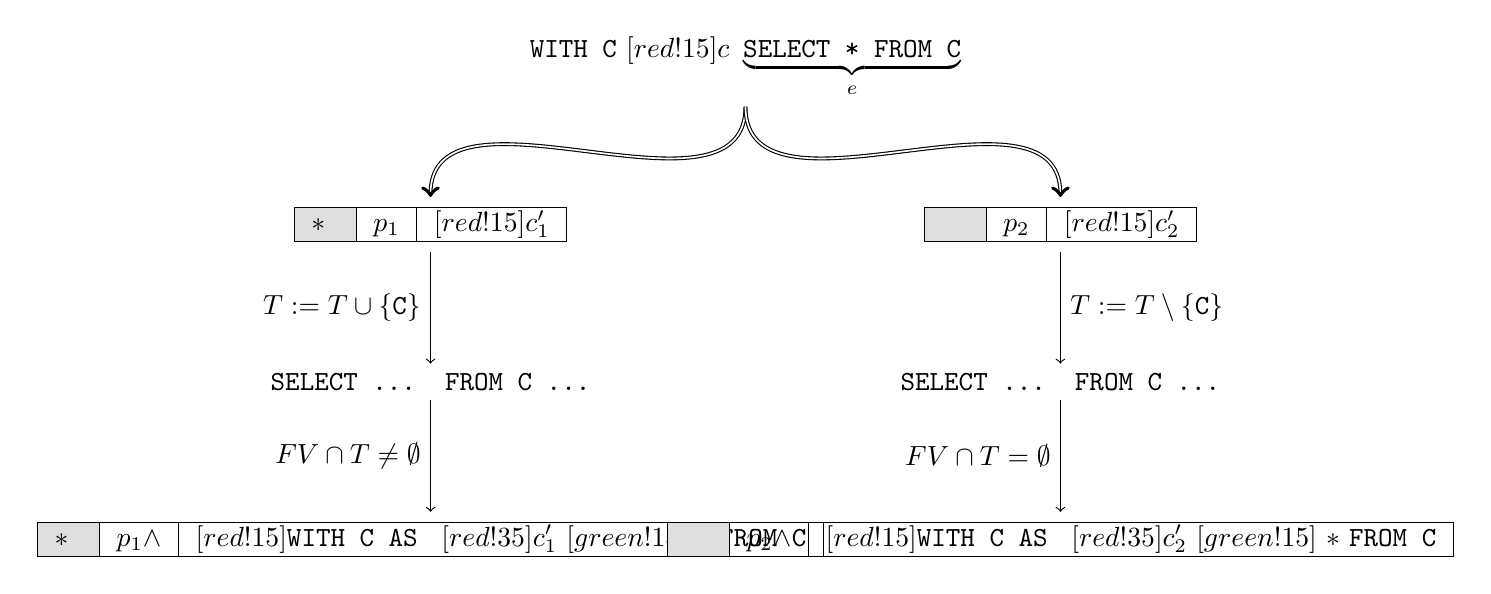
\begin{tikzpicture}
    \node (cte) at (4, 1) {\texttt{WITH C} \AS $\highlight[red!15]{c}~ \underbrace{\texttt{SELECT * FROM C}}_e$};
    \node (cte1) at (0, -1) {
        \begin{tabular}{|p{1em}|r|c|}\hline
        \cellcolor{gray!25} $\ast$ & $p_1$ & $\highlight[red!15]{c'_1}$\\\hline
        \end{tabular}
    };
    \node (cte2) at (8, -1) {
        \begin{tabular}{|p{1em}|r|c|}\hline
        \cellcolor{gray!25} & $p_2$ & $\highlight[red!15]{c'_2}$\\\hline
        \end{tabular}
    };
    \node (select1) at (0, -3) {\texttt{SELECT ... FROM C ...}};
    \node (select2) at (8, -3) {\texttt{SELECT ... FROM C ...}};
    \node (r1) at (0, -5) {
        \begin{tabular}{|p{1em}|r|c|}\hline
        \cellcolor{gray!25} $\ast$ & $p_1 \land \hdots$ & $\highlight[red!15]{\texttt{WITH C AS } ~\highlight[red!35]{c'_1}}~\highlight[green!15]{\SELECT~*~\texttt{FROM C}}$\\\hline
        \end{tabular}
    };
    \node (r2) at (8, -5) {
        \begin{tabular}{|p{1em}|r|c|}\hline
        \cellcolor{gray!25} & $p_2 \land \hdots$ & $\highlight[red!15]{\texttt{WITH C AS } ~\highlight[red!35]{c'_2}}~\highlight[green!15]{\SELECT~*~\texttt{FROM C}}$\\\hline
        \end{tabular}
    };
    \draw[->, double, out=270, in=90] (cte) to (cte1.north);
    \draw[->, double, out=270, in=90] (cte) to (cte2.north);
    \draw[->] (cte1.south) --node[left] {$T := T \cup \{\texttt{C}\}$} (select1);
    \draw[->] (cte2.south) --node[right]{$T := T \setminus \{\texttt{C}\}$} (select2);
    \draw[->] (select1) --node[left] {$FV \cap T \neq \emptyset$} (r1);
    \draw[->] (select2) --node[left] {$FV \cap T = \emptyset$} (r2);
    \end{tikzpicture}
    \caption{}
    \label{fig:my_label}
\end{figure}



\subsection{\RSELECT- and \RFROM-rule}


\begin{figure}[h!]\small
    \begin{minipage}[b]{.5\linewidth}
    \centering
    \sqlcode{snippets/fib_cte.sql}
    \subcaption{Fib with Ctes}\label{fib_cte_udf}
    \end{minipage}%
    \begin{minipage}[b]{.5\linewidth}
    \centering
     \begin{tikzpicture}
    \node[anchor=west] (s1) at (0, 0) {
        \begin{tabular}{|p{1em}|l|l|}\hline
        \cellcolor{gray!25}                         & \mintinline{sql}{TRUE AND} ~~ & ~~\mintinline{sql}{WITH C AS (SELECT 1)}\\
        \cellcolor{gray!25}\multirow{-2}{*}{} & \mintinline{sql}{n <= 2}   ~~ & ~~\mintinline{sql}{SELECT (SELECT P.i FROM P)}\\\hline
        \end{tabular}
    };
    \node[anchor=west, below=of s1] (s2) {
        \begin{tabular}{|p{1em}|l|l|}\hline
        \cellcolor{gray!25}                         & \mintinline{sql}{TRUE AND}   ~~ & ~~\mintinline{sql}{WITH C AS (SELECT 1)}\\
        \cellcolor{gray!25}                         & \mintinline{sql}{n <> 3 AND }~~ & ~~\mintinline{sql}{     S(i) AS (SELECT fib_cte3(n-2))}\\
        \cellcolor{gray!25}\multirow{-3}{*}{$\ast$} & \mintinline{sql}{NOT n <= 2} ~~ & ~~\mintinline{sql}{SELECT (SELECT T.i + S.i FROM S, T)}\\\hline
        \end{tabular}
    };
    \node[anchor=west, below=of s2] (s2) {
        \begin{tabular}{|p{1em}|l|l|}\hline
        \cellcolor{gray!25}                         & \mintinline{sql}{TRUE AND}      ~~ & ~~\mintinline{sql}{WITH C AS (SELECT 1)}\\
        \cellcolor{gray!25}                         & \mintinline{sql}{NOT n <> 3 AND}~~ & ~~\mintinline{sql}{     S(i) AS (SELECT 1)}\\
        \cellcolor{gray!25}\multirow{-3}{*}{$\ast$} & \mintinline{sql}{NOT n <= 2}    ~~ & ~~\mintinline{sql}{SELECT (SELECT T.i + S.i FROM S, T)}\\\hline
        \end{tabular}
    };
    \end{tikzpicture}
    \subcaption{Recursive scenarios}\label{fib_cte_scenarios}
    \end{minipage}
    \caption{}\label{fib_cte_translation}
\end{figure}





\iffalse OLD
$$\quad(\textsc{from})\inferrule{
    \exists i \in \{1, ..., n\}: T \vdash \hasCallsite(e_{f_i}) \\
    T[a_1 \mapsto \bot, ..., a_n \mapsto \bot] \vdash \neg \hasCallsite(e_s) \land \neg \hasCallsite(e_w) \\
    \forall i \in \{1, ..., n\}: T, \varnothing \vdash (\TRUE, t_i) \rightarrow (B_i, R_i)
}{
    T, \varnothing \vdash (p, \SELECT e_s \FROM t_1 \AS a_1 \otimes ... \otimes  t_n \AS a_n \WHERE e_w) \rightarrow \\\\
    {\begin{tabular}[b]{LLLL}
    (~~&\{&(&\SELECT p ~\AND~ p_1 ~\AND~ \cdots ~\AND~ p_n, \\
          &&&\SELECT e_s \FROM t'_1 \AS a_1 \otimes ... \otimes  t'_n \AS a_n \WHERE e_w ~~)\\
      && | &~((p_1, t'_1), ..., (p_n, t'_n)) \in \times_{\{i|1\leq i \leq n\}} B_i\}, \\
    &\{&(&\SELECT p_1 ~\AND~ \cdots ~\AND~ p_n, \\
       &&&\SELECT e_s \FROM t'_1 \AS a_1 \otimes ... \otimes  t'_n \AS a_n \WHERE e_w ~~)\\
       &&| &~ ((p_1, t'_1), ..., (p_n, t'_n)) \in \times_{\{i|1\leq i \leq n\}} (B_i \cup R_i), \exists t' \in \{t'_1, ..., t'_n\} : \hasCallsite(t')\})\\
    \end{tabular}}
}$$
\fi
$$\quad(\textsc{from})\inferrule{
    \exists i \in \{1, ..., n\}: \hasCallsite(T, e_{f_i}) \\
    \neg \hasCallsite(T, e_s)\\
    \neg \hasCallsite(T, e_w) \\\\
    \forall i \in \{1, ..., n\}: T, \varnothing \vdash (\TRUE, t_i) \rightarrow (B_i, R_i)
}{
    T, \varnothing \vdash (p, \SELECT~ e_s ~\FROM~ t_1 \AS a_1 \otimes ... \otimes  t_n \AS a_n ~\WHERE~ e_w) \rightarrow \\\\
    {\begin{tabular}[b]{LLLL}
    (~~&\{&(&\SELECT~ p ~\AND~ p_1 ~\AND~ \cdots ~\AND~ p_n, \\
          &&&\SELECT~ e_s ~\FROM~ t'_1 \AS a_1 \otimes ... \otimes  t'_n \AS a_n ~\WHERE~ e_w ~~)\\
      && | &~((p_1, t'_1), ..., (p_n, t'_n)) \in \times_{\{i|1\leq i \leq n\}} B_i\}, \\[6pt]
    &\{&(&\SELECT~ p_1 ~\AND~ \cdots ~\AND~ p_n, \\
       &&&\SELECT~ e_s ~\FROM~ t'_1 \AS a_1 \otimes ... \otimes  t'_n \AS a_n ~\WHERE~ e_w ~~)\\
       &&| &~ ((p_1, t'_1), ..., (p_n, t'_n)) \in \times_{\{i|1\leq i \leq n\}} (B_i \cup R_i), \exists t' \in \{t'_1, ..., t'_n\} : \hasCallsite(t')\}\\
    )\\
    \end{tabular}}
}$$

\subsection{\RCTE-rule: Collecting and analyzing CTE-Scenarios}
CTE-Scenarios are computed and dependencies for the scenarios are collected.
$$\quad(\textsc{cte})\inferrule{
    \hasCallsite(T, \WITH a_1 \AS t_1, ..., a_n \AS t_n~q)\\
    T, \varnothing \vdash (p, t_1) \rightarrow (B, R) \\
    ((B \times \{\bot\}) \cup (R \times \{\top\})) = \{(p'_{t_1}, t'_1, r_{i_1}), ..., (p'_{t_k}, t'_k, r_k)\} = X\\
    \forall (p'_t, t', r_i) \in X: T[a_1 \mapsto r_i], C[a_1: (t', p'_t, FV^+(t')] \vdash (p, \WITH a_2 \AS t_2, ..., a_n \AS t_n~q) \rightarrow (B_i, R_i)
}{
    T, C \vdash (p, \WITH a_1 \AS t_1, ..., a_n \AS t_n~q) \rightarrow ((\cup_{1 \leq i \leq k} B_i), (\cup_{1 \leq j \leq k} R_j)\})
}$$

$$\quad(\textsc{cte})\inferrule{
    T \vdash \hasCallsite(\WITH~ a_1 \AS t_1, ..., a_n \AS t_n~q)\\
    T, \varnothing \vdash (p, t_1) \rightarrow (B, R) \\
    \forall (p'_t, t') \in B: T \setminus \{a_1\}, C[a_1: (t', p'_t, FV^+(t')] \vdash (p, \WITH~ a_2 \AS t_2, ..., a_n \AS t_n~q) \rightarrow (B_i, R_i) \\
    \forall (p'_t, t') \in R: T \cup \{a_1\}, C[a_1: (t', p'_t, FV^+(t')] \vdash (p, \WITH~ a_2 \AS t_2, ..., a_n \AS t_n~q) \rightarrow (B_j, R_j)
}{
    T, C \vdash (p, \WITH~ a_1 \AS t_1, ..., a_n \AS t_n~q) \rightarrow ((\cup_{1 \leq i \leq k} B_i) \cup (\cup_{1 \leq j \leq l} B_j), (\cup_{1 \leq j \leq k} R_j) \cup (\cup_{1 \leq j \leq l} R_j)\})
}$$

\sqlcode{snippets/from_shadowing.sql}
\subsection{\RWITH-rule: Attaching used CTEs only}
When all CTEs at a level are processed, the actual query is processed independently. The query contains none of the preceeding CTEs anymore, so that it is sufficient to analyze the current subtree together with the set $T$ of recursive CTEs in scope to decide whether a subtree is recursive.
$$\quad(\textsc{with})\inferrule{
    C \neq \varnothing\\
    T, \varnothing \vdash (p, q) \rightarrow (B, R)
}{
    T, C \vdash (p, \WITH q) \rightarrow \\\\
    {\begin{tabular}[b]{LLLL}
    (~~&\{&(&\WITH [a_i \AS t_i]^{(a_i, t_i) \in \sigma_{a, t}(q'_{ctePreds})}~\SELECT (\AND_{p_i \in \{p_q\} \cup \sigma_p(q'_{ctes})} p_i), \\
          &&&\WITH [a_i \AS t_i]^{(a_i, t_i) \in \sigma_{a, t}(q'_{ctes})}~~q'~\\
          &&| &~(p_q, q') \in B,~ q'_{ctes} = C[FV^+(q')],~ q'_{ctePreds} = C[\cup_{x_p \in \{p_q\} \cup \sigma_p(q'_{ctes})} FV^+(x_p)]\},\\
    &\{&(&\WITH [a_i \AS t_i]^{(a_i, t_i) \in \sigma_{a, t}(q'_{ctePreds})}~\SELECT (\AND_{p_i \in \{p_q\} \cup \sigma_p(q'_{ctes})} p_i), \\
    &&&\WITH [a_i \AS t_i]^{(a_i, t_i) \in \sigma_{a, t}(q'_{ctes})}~~q'~\\
    &&|&~(p_q, q') \in R,~ q'_{ctes} = C[FV^+(q')],~ q'_{ctePreds} = C[\cup_{x_p \in \{p_q\} \cup \sigma_p(q'_{ctes})} FV^+(x_p)])
    \end{tabular}}
}$$
\\

% REF
$$\quad(\textsc{ref})\inferrule{
   \text{isReference}(S) \\
   T \vdash \hasCallsite(S)
}{
    T, C \vdash (p, S) \rightarrow (\{\}, \{(p, S)\})
}$$


\section{Postprocessing of the scenarios}
\subsection{Extraction of callsite-arguments}
We need to extract the arguments of the callsites within a recursive case, eg: 
\begin{minted}{sql}
SELECT T.a + T.b + T.c FROM (SELECT f(n-1, 2), 3, 4 + f(5, 6) FROM T WHERE p) AS T(a, b, c)
\end{minted}
into a set of callsite-arguments with its arguments $\{(\SELECT n-1, \SELECT 2), (\SELECT 5, \SELECT 6)\}$. As we require the callsite-arguments to be uncorrelated, we do not have to deal with references to \FROM but only to CTEs, wich simplifies things greatly.

Remove sourrinding query if callsite is within \SELECT, because the value of the callsite-arguments must be invariant to the tables references in \FROM.
$$\quad(\textsc{select})\inferrule{
    \exists i \in \{1, ..., n\}: \text{containsCallsite}(s_i) \\
    \forall i \in \{1, ..., n\}: \varnothing \vdash s_i \rightarrow P_i
}{
    \varnothing \vdash \SELECT s_1, ..., s_n \FROM f \WHERE w \rightarrow \\\\
    \{(\SELECT e_1, ..., \SELECT e_k) | (e_1, ..., e_k) \in \cup_{i \in \{1, ..., n\}} P_i \}
}$$

Remove outer query if callsite is within FROM, because sourrounding query is irrelevant for evaluation of subqueries in FROM.
$$\quad(\textsc{from})\inferrule{
    \forall i_j \in \{i_1, ...., i_m\} \subseteq \{1, ..., n\}: \text{containsCallsite}(f_{i_j})\\
    \forall i_j \in \{i_1, ...., i_m\}: \varnothing \vdash f_{i_j} \rightarrow P_{i_j}
}{
    \varnothing \vdash \SELECT s \FROM a_1 \AS f_1 \otimes ... \otimes a_n \AS f_n \WHERE w \rightarrow \cup_{i \in \{1, ..., n\}} P_i
}$$

Evaluate CTEs seperately, keeping previous CTEs that are referenced, in the case that there are callsites inside CTEs. Saving also every CTE to the CTE-store if they are references form the actual query.
$$\quad(\textsc{cte})\inferrule{
    \varnothing \vdash t_1 \rightarrow P \\
    C[a_1 : (t_1, FV^+(C, t_1))] \vdash \WITH a_2 \AS t_2, ..., a_n \AS t_n ~q \rightarrow P_w
}{
    C \vdash \WITH a_1 \AS t_1, ..., a_n \AS t_n ~q \rightarrow \\\\
    \{(\WITH [a_i \AS t_i]_{(a_i, t_i) \in C[FV^+(e_1)]} ~e_1, ..., \WITH [a_i \AS t_i]_{(a_i, t_i) \in C[FV^+(e_m)]} ~e_m) | (e_1, ..., e_m) \in P\} \cup P_w
}$$


$$\quad(\textsc{with})\inferrule{
    \varnothing \vdash q \rightarrow P
}{
    C \vdash \WITH q \rightarrow \\\\
    \{(\WITH [a_i \AS t_i]_{(a_i, t_i) \in C[FV^+(e)]} ~e_1, ..., \WITH [a_i \AS t_i]_{(a_i, t_i) \in C[FV^+(e_m)]} ~e_m) | (e_1, ..., e_m) \in P\}
}$$

Remove surrounding expression for every branch that contains a callsite, collecting results of all arguments.
$$\quad(\textsc{expr})\inferrule{
    \exists i \in \{1, ...., n\}: \text{containsCallsite}(e_i)\\
    \forall i \in \{1, ...., n\}: \varnothing \vdash e_i \rightarrow P_i
}{
    \varnothing \vdash \text{expr}(e_1, e_2, ..., e_n) \rightarrow \cup_{i \in \{1, ...., n\}} P_i
}$$

Remove recursive call and collect args.
$$\quad(\textsc{call})\inferrule{
}{
    \varnothing \vdash fn_{rec}(e_1, e_2, ..., e_n) \rightarrow \{ (e_1, e_2, ..., e_n) \}
}$$

If subbranch contains no callsite, stop and return empty set.
$$\quad(\textsc{nocall})\inferrule{
\neg \text{containsCallsite}(e)
}{  
    \varnothing \vdash e \rightarrow \{\}
}$$

Callsites within aggregate-functions are forbidden by the restriction that there must be a static number of callsites. Looping through a table, evaluating a recursive call per row is not allowed.





\chapter{Optimizations}

If certain characteristics of an UDF can be detected, the optimized translation templates can be chosen that exploits this characteristics. This may either improve performance or enables us to implement work-arounds for settings where the original templates are not applicable otherwise.

To make these optimizations no change in the scenario analysis is required. Instead, based on its output, ie. the generated scenarios, additionally analysis steps are performed to gather information required to choose the best templates.



\section{Single Recursion}

\begin{wrapfigure}{r}{0.2\textwidth}
  \vspace{-20pt}\centering
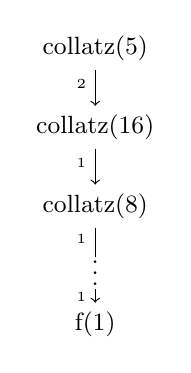
\begin{tikzpicture}\small
% nodes
\node (f1) at (0, 2) {collatz(5)};
\node (f2) at (0, 1) {collatz(16)};
\node (f3) at (0, 0) {collatz(8)};
\node (fn) at (0, -0.75) {$\vdots$};
\node (f0) at (0, -1.5) {f(1)};
% arrows
\draw[->] (f1) --node[pos=0.4, left, label distance=5mm]{\tiny{2}} (f2);
\draw[->] (f2) --node[pos=0.4, left, label distance=5mm]{\tiny{1}} (f3);
\draw (f3) --node[pos=0.4, left, label distance=5mm]{\tiny{1}} +(0, -0.65);
\draw[<-] (f0) --node[pos=0.4, left, label distance=5mm]{\tiny{1}} +(0, 0.45);
\end{tikzpicture}
  \vspace{-10pt}
  \caption{Callgraph of \texttt{collatz(5)}}
  \label{tr_callgraph}
\end{wrapfigure}

Single recursive functions have a linear branching behaviour (\autoref{tr_callgraph}). The function as a whole may contain multiple callsites as long as during evaluation each invocation will cause at most one recursive call. With the scenarios of the analysis, a single recursive function is quickly detected: If each scenario contains exactly one (or none) callsites, the function is single recursive.
The function that computed the length of the \textit{collatz-series} (\autoref{lst:collatz_udf}) is an example for a single recursive function.

\begin{figure}[h]
    \centering
    \begin{minipage}[b]{.45\linewidth}
    \centering
    \sqlcode{snippets/collatz.sql}
    \subcaption{UDf computing the length of the \textit{collatz-series} for a start number $\texttt{n} > 0$.}
    \label{lst:collatz_udf}
    \end{minipage}
    \begin{minipage}[b]{.5\linewidth}
    \centering\scriptsize
        \begin{tabular}{|p{1em}|p{3.3cm}|p{2.9cm}|}\hline
        \cellcolor{gray!25} & \texttt{\phantom{NOT }n=1} & \texttt{1}\\\hline
        \end{tabular}
        
        \begin{tabular}{|p{1em}|p{3.3cm}|p{2.9cm}|}\hline
        \cellcolor{gray!25} $\ast$ & \texttt{NOT n=1 AND \phantom{NOT }n \% 2 = 0} & \texttt{1 + collatz(n / 2)}\\\hline
        \end{tabular}
        
        \begin{tabular}{|p{1em}|p{3.3cm}|p{2.9cm}|}\hline
        \cellcolor{gray!25} $\ast$ & \texttt{NOT n=1 AND NOT n \% 2 = 0} & \texttt{1 + collatz(3 * n + 1)}\\\hline
        \end{tabular}
        \vspace{2em}
    \subcaption{Scenarios of \texttt{collatz}. Each recursive scenario contains just a single callsite.}\label{collatz_scenarios}
    \end{minipage}
    \caption{}
    \label{collatz_sql_with_scenarios}
\end{figure}

The evaluation happens thus also in a strict linear manner. As each scenario depends only on the result of the previous result, the work-around (see \autoref{macro:evaluation_cte}) to access all previous computed results becomes unnecessary. In each iteration exactly one result is computed and in the next iteration the dependant scenario will be evaluated. No need to add all previous results to the current result to have those rows later available (\autoref{opt_sr_evaluation_cte}). This has the very nice effect, that the intermediate-table of the \texttt{evaluation}-CTE does not grow quadratic (see \autoref{}) but only linear. Only actually new rows are added to the results.

\begin{figure}[h!]
    \centering
    \begin{minted}{postgresql}
WITH RECRUSIVE
    ...
    evaluation(in_1, res) AS (
        (TABLE basecases)
        
        UNION ( -- was UNION ALL
            WITH e AS (TABLE evaluation)
            (<evaluate recursive scenario_sr(scenario[1])>)
               UNION ALL
            (<evaluate recursive scenario_sr(scenario[2])>)
        )
    )
SELECT ...
    \end{minted}
    \caption{Simplified evaluation-template for single recursive UDFs.}
    \label{opt_sr_evaluation_cte}
\end{figure}

Furthermore, the rather complicated relational division, pivoting and filtering for evaluable scenarios (\autoref{macro:recursive_scenario_evaluation}) can be replaced by a much simpler query (\autoref{opt_sr_eval_scenario}). Because each scenario has only a single callsite, no grouping/partitioning is required to collect results of dependant callsites and to check whether all dependencies are available. If a result of the callsite is present, the scenario can be evaluated. What remains is basically a simple join (\autoref{opt_sr}).

\begin{figure}[h!]
    \centering
    \sqlcode{snippets/opt_sr.sql}
    \caption{Simplified macro for single recursive UDFs. Note how the \texttt{FROM}-clause is just a simple join and no \texttt{WHERE} is required anymore.}
    \label{opt_sr_eval_scenario}
\end{figure}





\section{Tail Recursion}
\begin{wrapfigure}{r}{0.5\textwidth}
  \vspace{-10pt}
    \sqlcode{snippets/collatz_tr.sql}
  \caption{Tail recursive formulation of \texttt{collatz}}
  \label{lst:fib_tr}
\end{wrapfigure}

A special form of single recursive functions are tail recursive functions. They do not have any evaluation context around any callsite so that each recursive scenario just returns another recursive call. Eventually, the result of the basecase is just passed all the way up in the callgraph to the root without any modifications. This last phase can therefore be skipped, which means that no \texttt{evaluation}-CTE is required.

The final result is present in the \texttt{basecase}-CTE. The basecase-CTE contains only a single value because single recursive functions have no branches in the callgraph (cp. \autoref{tr_callgraph}). The modifications on the template amount to removing the \texttt{evaluation}-CTE and changing result selection as shown in \autoref{tr_opt_template}. Furthermore the \texttt{callsite\_id}-column can be removed from the \texttt{callgraph}-CTE because the only use of the \texttt{callsite\_id} is to identify the corresponding scenario during evaluation (\autoref{marco:collect_call_maybe_optimized}).

\begin{figure}
    \centering
    \sqlcode{snippets/opt_tr.sql}
    \caption{Template for tail recursive UDFs. No \texttt{evaluation}-CTE is required anymore as all the basecases already return the final result.}
    \label{tr_opt_template}
\end{figure}


\begin{figure}[h!]\centering\small
    \begin{minted}{sql}
    <collect_call_maybe(in_arg_1, predicate, callsite)>
        := SELECT
             in_arg_1                    AS in_1, 
           --callsite.id                 AS callsite_id,
             callsite.arg_1[in_arg_1/$1] AS out_1
           FROM predicate AS p(is_true)
           WHERE p.is_true
    \end{minted}
  \caption{Pseudocode to generate a single call to the callstack-table, optimized for tail recursive UDFs. The callsite id is no longer required as the evaluation-phase is skipped.}
  \label{marco:collect_call_maybe_optimized}
\end{figure}

The detection if tail recursive functions happens again by inspecting the generated scenarios. The only callsite \texttt{f(...} must be present at the top level of the query of every scenario or nested arbitrarily deep in trivial \texttt{SELECT}s.
Nothing else may be present in the query as it would add a context that need to be saved and later on evaluated. Any computations like \texttt{1+(SELECT f(n))} would create a context around the call that need to be evaluated. The same for \FROM, even if the callsite-arguments contain no table-references, we are required to loop through the rows and create the output table.
\begin{figure}
    \centering
\begin{minted}{postgresql}
q := f(...)
q := (SELECT <c>)
q := (WITH [<alias> AS (<nonrecursive sql>), ...] <q>)
\end{minted}
    \caption{Grammar for tail-recursive queries. This notion could be extended, but catches most cases as it is.}
    \label{tr_grammar}
\end{figure}

CTEs are the only exception. If one of the callsite arguments reference a CTE and therefore the query is preceded by a \WITH-block, the function is still considered tail recursive. Callsite-arguments are evaluated during callgraph discovery. During evaluation the callsites, including their arguments, are replaced by references to their results. So, during evaluation, the CTEs are present but not used and could be therefore discarded. The resulting query is eligible for the tail recursive optimization.

\section{Constant parameter removal}

Unused parameters are always omitted.

Sometimes arguments are passed to functions that are invariant in subsequent calls, eg. configuration parameters. As these parameters do not change, it is not necessary to include them in the callgraph-table or to include them when matching rows by arguments. The argument can just be left as it is in the translation, eg. as \texttt{\$1}.

\begin{wrapfigure}{r}{0.66\textwidth}
  \vspace{-10pt}
    \sqlcode{snippets/sieve.sql}
  \caption{Sieve of Eratosthenes. \texttt{sieve(2, ARRAY[1, 2, 3, ..., n])} computes all prime numbers up to \texttt{n}.}
  \label{lst:sieve_udf}
\end{wrapfigure}

Removing unnecessary comparisons speeds up the query and saves memory as the same value is not copied again and again. The speedup can be significant, eg. in the function \texttt{sieve} (\autoref{lst:sieve_udf}). The function implements the sieve of Erathostenes, which filters out all non-prime numbers from a number array.

No change to the template is necessary and detection of constant arguments is straight-forward. The input is just removed from the list of arguments so that the argument is "not seen" when the templates are filled. The nth argument of a UDF is constant if the nth argument in each callsite is just \texttt{\$n}.

\begin{figure}[h]
    \centering\footnotesize
    \begin{minipage}[b]{\linewidth}
    \centering
    \begin{tabular}{c|c|c|c|c}
         in\_1 & in\_2                                     & callsite\_id & out\_1 & out\_2                                  \\\hline
         2     & \mintinline{postgresql}{ARRAY[2, 3, ..., 7]} & 1            & 3      & \mintinline{postgresql}{ARRAY[2, 3, ..., 7]}\\
         3     & \mintinline{postgresql}{ARRAY[2, 3, ..., 7]} & 1            & 4      & \mintinline{postgresql}{ARRAY[2, 3, ..., 7]}\\
    \end{tabular}
    \subcaption{\texttt{callgraph}-CTE for \texttt{sieve} without optimization}
    \label{}
    \end{minipage}
    \vspace{5mm}
    \begin{minipage}[b]{\linewidth}
    \centering
    \begin{tabular}{c|c|c}
         in\_1 & in\_2                                     & result                                  \\\hline
         4     & \mintinline{postgresql}{ARRAY[2, 3, ..., 7]} & \mintinline{postgresql}{ARRAY[2, 3, 4, 5, 6, 7]}\\
         3     & \mintinline{postgresql}{ARRAY[2, 3, ..., 7]} & \mintinline{postgresql}{ARRAY[2, 3, 4, 5, 7]}\\
         2     & \mintinline{postgresql}{ARRAY[2, 3, ..., 7]} & \mintinline{postgresql}{ARRAY[2, 3, 5, 7]}\\
    \end{tabular}
    \subcaption{\texttt{evaluation}-CTE for \texttt{sieve} without optimization}
    \label{}
    \end{minipage}
    \caption{}
    \label{}
\end{figure}

\begin{figure}[h]
    \centering
    \begin{minipage}[b]{.45\linewidth}
    \centering
    \begin{minted}{postgresql}
SELECT
    c.out_1      AS in_1, 
    c.out_2      AS in_2, 
    1            AS callsite_id,
    c.out_1 + 1  AS out_1
    c.out_2      AS out_2
FROM pred_1 AS p(is_true)
WHERE p.is_true
    \end{minted}
    \subcaption{\texttt{collect\_call\_maybe} without optimization}
    \label{}
    \end{minipage}
    \hfill
    \begin{minipage}[b]{.45\linewidth}
    \centering
    \begin{minted}{postgresql}
SELECT
    c.out_1      AS in_1, 
    1            AS callsite_id,
    c.out_1 + 1  AS out_1
FROM pred_1 AS p(is_true)
WHERE p.is_true
    \end{minted}
    \subcaption{\texttt{collect\_call\_maybe} with constant parameter removed}
    \label{}
    \end{minipage}
    \caption{Collection of a single scenario inside the \texttt{callgraph}-CTE.}
    \label{}
\end{figure}

\begin{figure}
    \centering
    \begin{minted}{postgresql}
SELECT c.in_1                                  AS in_1, 
       (SELECT array_agg(T.v)
        FROM unnest($2) AS T(v)
        WHERE (T.v = c.in_1 OR T.v % c.in_1 <> 0)
          AND T.v = ANY((SELECT e.result)))       AS result
FROM calls_to_basecases c
WHERE (SELECT (2 * c.out_1) > (array_length($2, 1))
    \end{minted}
    \caption{Evaluation of a nonrecursive scenario of \texttt{sieve} inside the \texttt{basecases}-CTE with constant parameter removed: \texttt{\$2} is not replaced by \texttt{c.in\_2}.}
    \label{fig:my_label}
\end{figure}

\section{Handling unhashable types}
The limitation to require hashability on input arguments of the UDF can be lifted if we implement measures to work around this issues. This lead to a greater applicability but is not desirable in the general case where this costly workaround is not necessary.


Hashable arguments
Hashable return value